%==============================================================================
%  PolySignal --- Technical Report
%  Social Media Signals and Prediction Market Outcomes: A Study on Polymarket
%  Big Data Engineering 2025/2026 --- Social Network Analysis, Track 2
%
%  Compile with pdfLaTeX:
%     pdflatex main
%     bibtex   main
%     pdflatex main
%     pdflatex main
%  (or simply use latexmk -pdf main.tex, or upload the pdf_latex/ folder to
%   Overleaf and press Recompile).
%==============================================================================
\documentclass[11pt,a4paper]{report}

%------------------------------------------------ encoding & fonts
\usepackage[T1]{fontenc}
\usepackage[utf8]{inputenc}
\usepackage{lmodern}
\usepackage{microtype}

%------------------------------------------------ layout
\usepackage[a4paper,margin=2.6cm,headheight=14pt]{geometry}
\usepackage{setspace}
\onehalfspacing
\usepackage{emptypage}

%------------------------------------------------ math & symbols
\usepackage{amsmath,amssymb,amsfonts}
\usepackage{bm}

%------------------------------------------------ graphics, tables, color
\usepackage{graphicx}
\graphicspath{{figures/}}
\usepackage{booktabs}
\usepackage{array}
\usepackage{multirow}
\usepackage{tabularx}
\usepackage{xcolor}
\usepackage{colortbl}
\usepackage{caption}
\usepackage{subcaption}
\usepackage{float}

%------------------------------------------------ lists, misc
\usepackage{enumitem}
\setlist{nosep,leftmargin=1.4em}
\usepackage{fancyhdr}
\usepackage{tikz}
\usetikzlibrary{arrows.meta,positioning,shapes.geometric,fit,backgrounds,calc}

%------------------------------------------------ palette (matches the figures)
\definecolor{psblue}{HTML}{3B6EA5}
\definecolor{psorange}{HTML}{C46A1F}
\definecolor{psgreen}{HTML}{4F8A4F}
\definecolor{psred}{HTML}{A83232}
\definecolor{pspurple}{HTML}{6D5B97}
\definecolor{psgrey}{HTML}{5A5A5A}
\definecolor{pslight}{HTML}{EEF2F7}
\definecolor{pslightgrey}{HTML}{F4F4F4}

%------------------------------------------------ hyperlinks
\usepackage[hidelinks,breaklinks=true]{hyperref}
\hypersetup{
  colorlinks=true, linkcolor=psblue, citecolor=psgreen,
  urlcolor=psblue, pdftitle={PolySignal --- Technical Report},
  pdfauthor={Francesco Simone Pirozzi, Gerardo Lauro}}
\usepackage[nameinlink]{cleveref}

%------------------------------------------------ bibliography
\usepackage[numbers,sort&compress]{natbib}
\bibliographystyle{plainnat}

%------------------------------------------------ chapter / section styling
\usepackage{titlesec}
\titleformat{\chapter}[display]
  {\normalfont\sffamily\bfseries}
  {\color{psgrey}\large CHAPTER \thechapter}
  {6pt}
  {\Huge\color{psblue}}
\titlespacing*{\chapter}{0pt}{-18pt}{22pt}
\titleformat{\section}
  {\normalfont\sffamily\large\bfseries\color{psblue!85!black}}{\thesection}{0.7em}{}
\titleformat{\subsection}
  {\normalfont\sffamily\normalsize\bfseries\color{psgrey}}{\thesubsection}{0.6em}{}

%------------------------------------------------ headers / footers
\pagestyle{fancy}
\fancyhf{}
\renewcommand{\headrulewidth}{0.3pt}
\fancyhead[L]{\footnotesize\sffamily\nouppercase{\leftmark}}
\fancyhead[R]{\footnotesize\sffamily PolySignal}
\fancyfoot[C]{\thepage}
\renewcommand{\chaptermark}[1]{\markboth{\thechapter.\ #1}{}}

%------------------------------------------------ caption style
\captionsetup{font=small,labelfont={bf,color=psblue},labelsep=period}
\captionsetup[sub]{font=small,labelfont=bf}

%------------------------------------------------ handy macros
\newcommand{\code}[1]{\texttt{\small #1}}
\newcommand{\unit}[1]{\,\mathrm{#1}}
\newcommand{\pyes}{p_{\text{YES}}}
\newcommand{\pmarket}{p_{m}}
\newcommand{\psocial}{p_{s}}
\newcommand{\keyfinding}[1]{%
  \begin{center}\colorbox{pslight}{\parbox{0.93\linewidth}{\small #1}}\end{center}}

% a light "callout" box for take-aways
\newenvironment{takeaway}
  {\par\smallskip\noindent\begin{tabular}{@{}p{0.012\linewidth}p{0.93\linewidth}@{}}
   \textcolor{psorange}{\rule{2pt}{\baselineskip}} &}
  {\end{tabular}\par\smallskip}

% allow TeX a little extra slack on hard-to-break lines (long \texttt filenames,
% ``a+b+c''-style feature strings) so they never spill into the margin
\setlength{\emergencystretch}{3em}

%==============================================================================
\begin{document}

%------------------------------------------------ TITLE PAGE
\begin{titlepage}
\centering
\vspace*{1.2cm}
{\sffamily\small Big Data Engineering --- A.Y. 2025/2026\par}
{\sffamily\small Social Network Analysis Challenge, Track 2\par}
\vspace{1.4cm}

{\sffamily\bfseries\color{psblue}\Huge PolySignal\par}
\vspace{0.5cm}
{\sffamily\Large A Social--Intelligence Layer for\\[2pt] Polymarket Prediction Markets\par}
\vspace{0.9cm}
{\itshape\large Social Media Signals and Prediction Market Outcomes:\\ a data-driven study on Polymarket\par}

\vspace{1.6cm}
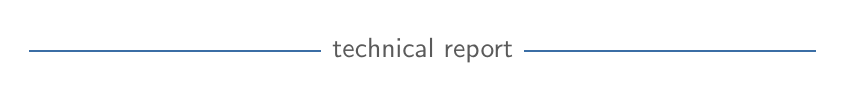
\begin{tikzpicture}
\draw[psblue,line width=1pt] (0,0) -- (10,0);
\node[fill=white,inner sep=4pt] at (5,0)
  {\sffamily\color{psgrey} technical report};
\end{tikzpicture}

\vspace{1.4cm}
{\large\sffamily\bfseries Francesco Simone Pirozzi \quad\textbullet\quad Gerardo Lauro\par}
\vspace{0.4cm}
{\sffamily\small Course instructor: Prof.\ Vincenzo Moscato\par}

\vfill

\begin{minipage}{0.86\linewidth}
\small\itshape\color{psgrey}\centering
\textbf{Research question.} Do social-media signals provide incremental
predictive value over market-implied probabilities, across thematic domains,
platforms, and time windows? We answer it with a reproducible, leakage-controlled
pipeline over 300~resolved Polymarket contracts and a corpus of
${\sim}1.36$~million social-media posts.
\end{minipage}

\vspace{1.0cm}
{\sffamily\small June 2026\par}
\end{titlepage}

%------------------------------------------------ ABSTRACT
\thispagestyle{empty}
\chapter*{Abstract}
\addcontentsline{toc}{chapter}{Abstract}
\markboth{Abstract}{}
\noindent
Prediction markets such as Polymarket aggregate the beliefs of many traders into a
single, continuously updated probability of a future event. Social-media platforms,
in parallel, host the public discourse through which those beliefs form. This report
studies, empirically and conservatively, whether that discourse carries information
that is \emph{not already priced in} by the market.

We build an end-to-end Big Data pipeline that (i)~collects \textbf{300 resolved
binary Polymarket contracts}, balanced across politics, finance, and sports
(100 each), together with their \textbf{full-lifetime price series}
(1{,}353{,}114 price points); (ii)~collects a longitudinal social corpus of
\textbf{1{,}368{,}041 posts} through source-appropriate collectors for the
\textbf{three platforms} named by the assignment --- Telegram (MTProto), Reddit
(public-web), and X/Twitter (authenticated automation), \textbf{all three present in
the analysed corpus}. Telegram dominates (98.6\%), Reddit is secondary (1.2\%), and
X/Twitter is a small but real third platform (2{,}822 posts, 0.2\%) whose scale is
capped by X's anti-automation defences --- a limitation we document rather than paper
over (\Cref{sec:scope}); (iii)~links posts to
contracts with a deterministic semantic-relevance scorer; (iv)~enriches the text
with sentiment, named entities, hashtags, language detection, and topic models;
(v)~projects the result into a Neo4j knowledge graph; and (vi)~derives a per-market
\emph{Social Pressure Index} that feeds a leakage-controlled backtest.

The descriptive analysis confirms textbook market behaviour: market-implied
probabilities are already strongly informative of the final outcome, and become
monotonically more so as resolution approaches (AUC rising from $0.90$ at
90~days to $0.99$ at close). The predictive study delivers a clear and honest
\textbf{null result}: a market-only model attains a Brier score of $0.031$ and
AUC $0.989$, whereas adding social features \emph{degrades} performance
($\Delta\text{Brier}=+0.009$), and a social-only model is no better than chance
(AUC $0.404$). We trace this to three structural causes --- a hype/optimism bias in
social discourse, a coverage mismatch between the available channels and the market
sample, and the informational efficiency of the market price itself --- and we argue
that this negative result is a meaningful empirical contribution rather than a
failure. All findings are exposed through an interactive \textbf{React} dashboard
served from a local, zero-dependency API.

\medskip
\noindent\textit{\small Reproducibility note. Every quantitative result in this report is
regenerated from the persisted pipeline artifacts by a single released step
(\code{python scripts/\_paper\_figs.py}), so the figures and tables always match the
dataset on disk and no number is hand-transcribed.}

\tableofcontents
\listoftables

%------------------------------------------------ BODY
%==============================================================================
%  PART 1 --- FOUNDATIONS
%  Chapters: Introduction | Background & Related Work | Data Model & Dataset
%==============================================================================

\chapter{Introduction}
\label{ch:intro}

\section{Context and motivation}
Prediction markets are exchanges on which participants trade contracts whose
payoff is tied to the outcome of a future, verifiable event. Because a rational
trader buys a ``\textsc{Yes}'' share whenever its price is below their subjective
probability of the event and sells when it is above, the equilibrium price of a
binary contract behaves as a continuously updated, money-weighted estimate of the
event's probability~\cite{wolfers2004prediction,berg2008prediction}. Among
contemporary platforms, \emph{Polymarket} has become one of the most liquid and
widely watched venues, hosting contracts on politics, macroeconomics, crypto-asset
price levels, sports, and current affairs. The resolved history of these contracts
provides something rare in forecasting research: a large set of events with a
\emph{known ground-truth outcome} and a \emph{full price trajectory} leading up to
it.

In parallel, a large share of the public reasoning \emph{about} these same events
happens on social-media platforms --- Reddit threads, Telegram channels, and posts
on X (formerly Twitter). This discourse encodes sentiment, narratives, rumours, and
occasionally genuine private information. A long line of work has asked whether such
signals anticipate real-world or market outcomes, with results ranging from
optimistic~\cite{bollen2011twitter,salathe2012assessing} to sharply
qualified~\cite{tetlock2007giving}. The question is far from settled, and it is
exactly the question this project investigates in the specific, well-instrumented
setting of Polymarket.

\section{Research question and objectives}
The project is organised around a single, deliberately conservative research
question:

\keyfinding{\textbf{Do social-media signals provide \emph{incremental} predictive
value over market-implied probabilities, and if so, in which thematic domains, on
which platforms, and over which time windows?}}

\noindent The emphasis on \emph{incremental} value is the methodological core of the
work. It is easy --- and uninteresting --- to show that social sentiment correlates
with an outcome when the market price already encodes that information. The
scientifically meaningful test is whether social features improve a forecast
\emph{on top of} the market price, under an evaluation that forbids any leakage of
post-resolution information. We therefore frame PolySignal not as an attempt to
``beat Polymarket'', but as an analytical layer that quantifies social context and
submits it to a controlled, falsifiable test.

\noindent Operationally, the work pursues the three goals set out by the assignment:
\begin{enumerate}
  \item \textbf{Dataset construction (Task 1).} Build a reproducible ingestion
  pipeline that collects resolved Polymarket contracts and their price time series,
  collects longitudinal social discourse, links posts to contracts, normalises and
  enriches the text, and stores everything in a queryable format.
  \item \textbf{Analytical study (Task 2).} Characterise the contracts and the
  discourse descriptively; study the temporal relationship between social signals
  and price movements; compare platforms and domains; and expose the results through
  an interactive dashboard.
  \item \textbf{Outcome prediction (Task 3, optional).} Engineer social features and
  evaluate, with temporal cross-validation and explicit ablations, whether they add
  predictive value over the market price.
\end{enumerate}

\section{Design philosophy}
Four principles shaped every component and are worth stating up front, because they
explain many concrete choices later in the report.

\begin{description}[leftmargin=1.4em,style=nextline]
  \item[Deterministic core, optional intelligence.] The full pipeline runs
  end-to-end \emph{without} any call to an external language model. LLM-assisted
  steps exist only as opt-in, cached verifiers layered on top of a deterministic
  baseline. This guarantees reproducibility and decouples our results from a paid,
  non-deterministic dependency.
  \item[Time discipline and no leakage.] Every record carries a timezone-aware
  timestamp, and every forecasting or backtesting step enforces a strict
  ``no information from the future'' rule: a market's resolution can never reach a
  feature, and a post published after a contract closed can never count as evidence
  for it.
  \item[No invented data.] The system never fabricates posts, markets, or labels to
  inflate coverage. Empty or sparse cells are reported honestly --- a property that
  proves essential when we discuss the coverage limitations in
  \Cref{ch:limitations}.
  \item[Honest reporting.] We report a negative predictive result in full, with its
  diagnostics, rather than selecting a favourable slice. A robust null result, in a
  field prone to over-optimistic claims, is itself a contribution.
\end{description}

\section{Scope decisions}
\label{sec:scope}
Two scope decisions are load-bearing and are justified in detail where they arise;
we summarise them here so the reader can keep them in mind.

\paragraph{Platforms: all three collected, Telegram-dominated.}
The assignment names three platforms, and the pipeline implements a collector for
each: \textbf{Telegram} (via the official MTProto API, using Telethon),
\textbf{Reddit} (via compliant public-web scraping with Scrapling against
\code{old.reddit.com}, since we deliberately avoid the OAuth API), and
\textbf{X/Twitter} (via authenticated browser automation with Playwright, because X's
free programmatic tier no longer supports research collection). Each post, regardless
of source, is normalised into a single platform-agnostic \code{SocialPostRecord}, so
linking, enrichment, and evaluation never branch on platform. \textbf{All three
platforms are present in the analysed corpus}, but in sharply unequal volume: Telegram
dominates (98.6\%), Reddit is secondary (1.2\%), and X/Twitter is a small third
platform (2{,}822 posts, 0.2\%). X's anti-automation defences (token challenges, login
walls, aggressive rate limiting) cap how much can be gathered responsibly, so its
contribution is modest --- but it is genuine, and the cross-platform analysis of
\Cref{ch:crossplatform} is a real \textbf{three-platform} comparison (114 contracts
carry all three sources). The load-bearing caveat is therefore not that a platform is
missing but that the corpus is \textbf{Telegram-dominated and
crypto/macro/geopolitics-tilted}; we restate this wherever it bears on a result rather
than softening it.

\paragraph{Contracts: binary \textsc{Yes}/\textsc{No} only.}
We restrict the study to binary \textsc{Yes}/\textsc{No} contracts. Every downstream
component --- stance detection, the Social Pressure Index, the forecast blender, and
the backtest --- is natively two-outcome aware, and generalising to multi-outcome
markets would require changing all of them in lockstep. Binary contracts are also
the cleanest setting for the incremental-value question, since the target is a
single Bernoulli variable.

\section{Contributions}
This report contributes:
\begin{enumerate}
  \item a \textbf{reproducible Big Data pipeline} that turns two heterogeneous,
  high-volume sources (a prediction market and multi-platform social discourse) into
  a single, queryable, leakage-aware dataset of 300 resolved contracts and ${\sim}1.37$
  million posts;
  \item a \textbf{deterministic contract--post linking and outcome-aware stance}
  method that scales to hundreds of thousands of candidate pairs without an LLM in
  the loop;
  \item a per-market \textbf{Social Pressure Index} that condenses volume, stance,
  engagement, source diversity, and temporal dynamics into interpretable features;
  \item a \textbf{leakage-controlled backtest} with four baselines and an ablation
  that isolates the incremental value of social signals; and
  \item a careful, evidence-backed \textbf{negative result} together with a
  root-cause analysis explaining \emph{why} public social signals do not beat the
  market price in this setting.
\end{enumerate}

\section{Structure of the report}
The report is organised into four parts that follow the data as it flows through the
system. \textbf{Part~I} (this part) sets up the problem, the related work, and the
data model. \textbf{Part~II} describes the ingestion pipeline (Task~1): system
architecture and storage, data collection, contract--post linking, and text
enrichment. \textbf{Part~III} presents the analytical study (Task~2): descriptive
analysis of contracts and discourse, signal--market correlation, cross-platform
comparison, and the dashboard. \textbf{Part~IV} reports the predictive study
(Task~3), discusses why social signals fail to add value, states the limitations,
and concludes.


%==============================================================================
\chapter{Background and Related Work}
\label{ch:background}

\section{Prediction markets and informational efficiency}
The idea that a market price aggregates dispersed private information into a single
public statistic goes back to Hayek's argument that prices are society's mechanism for
pooling knowledge no individual holds in full~\cite{hayek1945use}. Modern prediction
markets operationalise this idea directly: the Iowa Electronic Markets have forecast
US election outcomes more accurately than polls across several
cycles~\cite{berg2008prediction}, and the broad survey of
Wolfers and Zitzewitz~\cite{wolfers2004prediction} documents the same pattern across
political, economic, and sports events. The theoretical appeal rests on the same
logic as the efficient-market hypothesis~\cite{fama1970efficient}: if a price fails to
reflect available information, an informed trader can profit by correcting it, and in
doing so moves the price. Empirically, prediction-market prices have been found to be
well-calibrated and hard to beat over long horizons~\cite{wolfers2004prediction,
berg2008prediction}. For our purposes this has a sharp methodological implication:
\emph{any} public signal that is genuinely predictive is also, by the same argument,
likely to be \emph{already incorporated} into the price. The bar for ``incremental
value'' is therefore high by construction, and a negative result is the theoretically
expected outcome unless the social signal carries information the market has not yet
absorbed (for instance, an early or private signal).

\section{Social media as a predictive signal}
The hypothesis that aggregate online sentiment anticipates collective outcomes was
popularised by Bollen et al.~\cite{bollen2011twitter}, who reported that Twitter mood
dimensions improved short-horizon stock-index forecasts, and by Salath\'e and
Khandelwal~\cite{salathe2012assessing} in the public-health domain. Tetlock's study
of media pessimism and the stock market~\cite{tetlock2007giving} is more cautionary:
he finds that media sentiment predicts \emph{temporary} price pressure that
subsequently reverts, consistent with sentiment proxying for noise rather than
fundamentals. The broader literature is mixed, and many positive findings have proven
fragile out of sample. PolySignal is designed precisely to avoid the methodological
traps --- look-ahead leakage, in-sample feature selection, and the conflation of
correlation with incremental value --- that produce fragile claims.

\section{Sentiment versus stance}
A recurring confusion in this literature is between \emph{sentiment} (the emotional
polarity of a text, independent of any target) and \emph{stance} (the directional
position of a text \emph{with respect to a specific proposition}). ``This is
terrible news for Iran'' is negative in sentiment but may \emph{support} the
\textsc{Yes} outcome of a contract such as ``Will Iran's regime fall?''. Because the
research question is about contract outcomes, we compute both: sentiment as a generic
descriptive feature (\Cref{ch:nlp}) and outcome-aware stance as the directional
signal that feeds prediction (\Cref{ch:nlp,ch:prediction}).

\section{Positioning}
Relative to prior work, this project is distinguished less by a novel model than by
\emph{methodological discipline at Big Data scale}: a heterogeneous,
million-row corpus; a transparent, deterministic linking and stance layer; a knowledge
graph as a queryable projection; and an evaluation whose leakage controls are explicit
and auditable. The headline result --- that public social signals do not add
incremental value here --- is consistent with the efficiency argument above and is
reported without embellishment.


%==============================================================================
\chapter{Data Model and Dataset Construction}
\label{ch:data}

The dataset has two interconnected components --- \textbf{Polymarket contract data}
and \textbf{social-media discourse data} --- collected, linked, and organised into a
single schema. This chapter defines that schema, maps it onto the fields required by
the assignment, and describes how the 300-contract study set was selected. The
mechanics of \emph{how} the data is collected and processed are deferred to
Part~II; here we specify \emph{what} the data is.

\section{The unified schema}
\label{sec:schema}
All normalised entities are stored as flat, typed tables (Apache Parquet; see
\Cref{ch:architecture} for the rationale). \Cref{tab:schema-market,tab:schema-post}
list the principal fields and show that every field required by the assignment is
present, alongside the derived, analysis-ready columns we add.

\begin{table}[H]
\centering
\caption[Contract and price-series schema]{Contract and price-series schema. The left
block lists the fields required by the assignment; the right block lists the value or
derivation in our dataset.}
\label{tab:schema-market}
\small
\begin{tabularx}{\linewidth}{@{}l l X@{}}
\toprule
\textbf{Required field} & \textbf{Our column} & \textbf{Notes / derivation}\\
\midrule
\multicolumn{3}{@{}l}{\textit{\code{markets.parquet}} --- one row per contract}\\
\addlinespace[2pt]
\code{market\_id}        & \code{market\_id}      & Polymarket \code{conditionId}\\
\code{question}          & \code{question}        & full question text\\
\code{category}          & \code{thematic\_category} & \{politics, finance, sports\}; plus a finer \code{domain}\\
\code{outcomes}          & \code{outcomes}        & binary \textsc{Yes}/\textsc{No}\\
\code{resolution\_outcome}& \code{resolution}      & \textsc{Yes}/\textsc{No} declared at settlement\\
\code{resolution\_date}  & \code{resolved\_at}    & UTC timestamp\\
\code{creation\_date}    & \code{created\_at}     & UTC timestamp\\
\code{close\_date}       & \code{close\_time}     & UTC timestamp\\
\code{url}               & \code{source\_url}     & canonical Polymarket URL\\
\addlinespace[2pt]
--- & \code{volume}, \code{liquidity} & trading volume and book liquidity (derived)\\
\midrule
\multicolumn{3}{@{}l}{\textit{\code{price\_points.parquet}} --- one row per (contract, outcome, timestamp)}\\
\addlinespace[2pt]
\code{market\_id}        & \code{market\_id}      & foreign key to the contract\\
\code{outcome}           & \code{outcome\_id}     & CLOB token id (\textsc{Yes}/\textsc{No})\\
\code{timestamp}         & \code{timestamp}       & UTC; full-lifetime, ${\sim}$hourly to daily\\
\code{price}             & \code{price}           & implied probability in $[0,1]$\\
\code{volume}            & \code{volume}          & cumulative volume where available\\
\bottomrule
\end{tabularx}
\end{table}

\begin{table}[H]
\centering
\caption[Social-post schema]{Social-post schema (\code{social\_posts.parquet} and the
derived \code{post\_enrichment.parquet}). ``available'' marks fields present where the
source exposes them.}
\label{tab:schema-post}
\small
\begin{tabularx}{\linewidth}{@{}l l X@{}}
\toprule
\textbf{Required field} & \textbf{Our column} & \textbf{Notes}\\
\midrule
\code{post\_id}            & \code{post\_id}                 & stable per-platform id\\
\code{platform}            & \code{platform}                 & \code{telegram} / \code{reddit} / \code{twitter}\\
\code{url}                 & \code{url}                      & canonical post URL\\
\code{market\_id}          & via \code{linked\_posts}        & semantic link (\Cref{ch:linking})\\
\code{search\_query}       & \code{query}, \code{query\_type}& query + generator type\\
\code{collected\_at}       & \code{collected\_at}            & retrieval timestamp\\
\code{category}            & inherited from contract         & through the link\\
\code{author\_id/name}     & \code{author\_id}, \code{author\_name} & available\\
\code{author\_followers}   & ---                             & not exposed by broadcast channels\\
\code{published\_at}       & \code{created\_at}              & UTC, normalised\\
\code{text}                & \code{text}, \code{title}       & full text\\
\code{hashtags}            & \code{hashtags}                 & regex-extracted (enrichment)\\
\code{mentioned\_entities} & \code{mentioned\_entities}      & NER (enrichment)\\
\code{language}            & \code{language}                 & detected (enrichment)\\
\code{like/reply/repost/view} & \code{engagement\_score}, \code{upvotes}, \code{comments\_count}, \dots & available per platform\\
\code{comments}            & \code{comments\_count}, \code{post\_comments} & counts always captured; a \emph{sample} of reply text + author + timestamp is collected by the comment collector (\Cref{sec:social-collection})\\
\bottomrule
\end{tabularx}
\end{table}

\section{The 300-contract study set}
\label{sec:studyset}
The assignment requires \emph{at least 100 resolved contracts per thematic domain}.
We assembled a \textbf{domain-balanced set of 300 resolved binary contracts ---
exactly 100 politics, 100 finance, and 100 sports} --- under the three-way
\code{thematic\_category} used throughout the report. Internally, Polymarket exposes
a finer six-value domain taxonomy; \Cref{tab:domain-map} shows how it maps to the
assignment's three buckets and the resulting composition of the study set.

\begin{table}[H]
\centering
\caption[Fine domain to thematic-category mapping]{Mapping from Polymarket's fine domain
taxonomy to the three thematic categories, with the composition of the 300-contract
study set.}
\label{tab:domain-map}
\small
\begin{tabular}{@{}l l r@{}}
\toprule
\textbf{Thematic category} & \textbf{Fine domains} & \textbf{Contracts}\\
\midrule
politics & politics, geopolitics & 100\\
finance  & crypto (56), economy/macro (44) & 100\\
sports   & sports (98), culture/entertainment (2) & 100\\
\midrule
\textbf{Total} & & \textbf{300}\\
\bottomrule
\end{tabular}
\end{table}

Each contract was required to be (i)~\emph{resolved}, so that the ground-truth outcome
is known; (ii)~\emph{binary} \textsc{Yes}/\textsc{No}; and (iii)~backed by a
\emph{verified full-lifetime price timeline} from creation to settlement. Contracts
without a usable price history were rejected and replaced rather than padded. The
resulting price store contains \textbf{1{,}353{,}114 price points} across all
300 contracts, with a median of \textbf{4{,}899} points per contract --- dense enough
to study intraday dynamics.

\Cref{fig:domain-res} summarises the study set. The resolution distribution is
strongly imbalanced: \textbf{243 contracts (81\%) resolved \textsc{No}} and only
\textbf{57 (19\%) resolved \textsc{Yes}}. This base rate is itself informative ---
most ``Will $X$ happen by date $D$?'' contracts describe salient but ultimately
low-probability events --- and it conditions the entire predictive analysis in
Part~IV.

\begin{figure}[H]
\centering
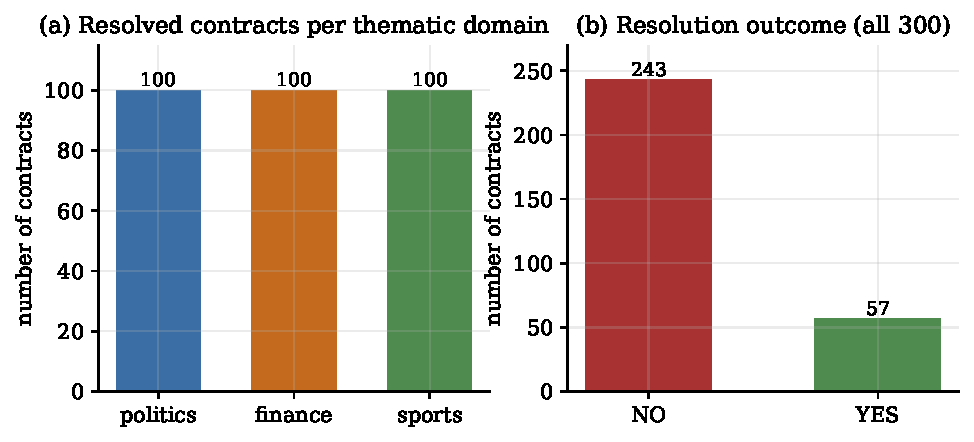
\includegraphics[width=\linewidth]{fig_domain_resolution.pdf}
\caption{The 300-contract study set. (a)~Exactly 100 resolved contracts per thematic
domain. (b)~The resolution outcome is heavily skewed towards \textsc{No}
(243 vs.\ 57), an imbalance that any predictive model must respect.}
\label{fig:domain-res}
\end{figure}

\section{Dataset at a glance}
\Cref{tab:glance} consolidates the headline figures of the constructed dataset; each
is derived in the chapters that follow. Together they make the scale concrete: two
heterogeneous sources, more than 2.7~million primary records before enrichment, and a
fully linked and labelled analytical layer on top.

\begin{table}[H]
\centering
\caption[The constructed dataset at a glance]{The constructed dataset at a glance.
Every figure is regenerated from the persisted pipeline artifacts
(\code{scripts/\_paper\_figs.py}).}
\label{tab:glance}
\small
\begin{tabular}{@{}l r l@{}}
\toprule
\textbf{Artifact} & \textbf{Count} & \textbf{Notes}\\
\midrule
Resolved binary contracts        & 300        & 100 / 100 / 100 by domain\\
Price points                     & 1{,}353{,}114 & full lifetime, 300/300 contracts\\
Social posts (deduplicated)      & 1{,}368{,}041 & Telegram 1{,}348{,}965 + Reddit 16{,}254 + X 2{,}822\\
Distinct channels / subreddits   & 68         & ---\\
Enriched posts                   & 1{,}368{,}041  & sentiment + NER + hashtags + language (all posts)\\
Scored contract--post pairs      & 4{,}112{,}547  & deterministic relevance\\
Accepted evidence links          & 37{,}562   & over 147 contracts\\
Outcome-aware stance labels      & 35{,}679   & over 140 contracts\\
LDA topics                       & 10         & over linked discourse\\
Knowledge-graph relationships    & $>2.7$M    & Neo4j projection\\
\bottomrule
\end{tabular}
\end{table}

%==============================================================================
%  PART 2 --- THE INGESTION PIPELINE (Task 1)
%  Chapters: Architecture & Storage | Data Ingestion | Linking | NLP Enrichment
%==============================================================================

\chapter{System Architecture and Storage}
\label{ch:architecture}

This chapter describes the architecture of the ingestion pipeline (Task~1) and
motivates the storage solution, which the assignment singles out as a graded design
choice.

\section{Architecture overview}
PolySignal is a sequence of loosely coupled modules, each with a typed input
contract, a typed output contract, and no knowledge of how its neighbours are
implemented. Data flows in one direction --- from external sources to the dashboard
--- and is persisted at every stage, so any stage can be re-run, audited, or replaced
in isolation. \Cref{fig:arch} shows the flow.

\begin{figure}[H]
\centering
\resizebox{\linewidth}{!}{%
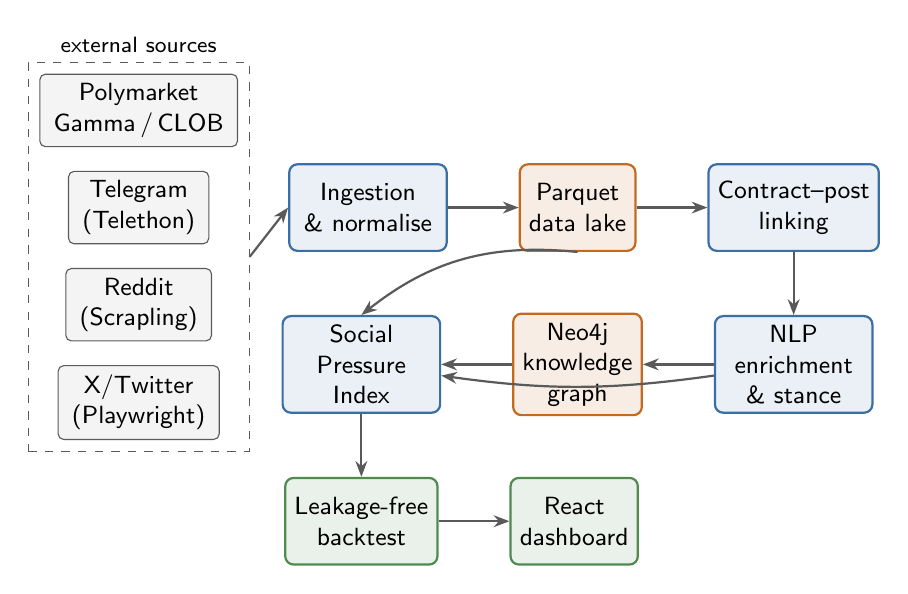
\begin{tikzpicture}[
  font=\sffamily\small,
  node distance=6mm and 9mm,
  src/.style={draw=psgrey,fill=pslightgrey,rounded corners=2pt,minimum height=8mm,inner xsep=5pt,align=center},
  stage/.style={draw=psblue,fill=psblue!10,rounded corners=3pt,minimum height=11mm,minimum width=20mm,align=center,thick},
  store/.style={draw=psorange,fill=psorange!12,rounded corners=3pt,minimum height=11mm,align=center,thick},
  result/.style={draw=psgreen,fill=psgreen!12,rounded corners=3pt,minimum height=11mm,align=center,thick},
  arr/.style={-{Stealth[length=2mm]},psgrey,thick}
]
% sources
\node[src] (poly) {Polymarket\\Gamma\,/\,CLOB};
\node[src,below=3mm of poly] (tg) {Telegram\\(Telethon)};
\node[src,below=3mm of tg] (rd) {Reddit\\(Scrapling)};
\node[src,below=3mm of rd] (x) {X/Twitter\\(Playwright)};
\node[draw=psgrey,dashed,fit=(poly)(tg)(rd)(x),inner sep=4pt,label=above:{\footnotesize external sources}] (sources) {};

\node[stage,right=10mm of tg] (ing) {Ingestion\\\& normalise};
\node[store,right=of ing] (parq) {Parquet\\data lake};
\node[stage,right=of parq] (link) {Contract--post\\linking};
\node[stage,below=8mm of link] (nlp) {NLP\\enrichment\\\& stance};
\node[store,left=of nlp] (graph) {Neo4j\\knowledge\\graph};
\node[stage,left=of graph] (feat) {Social\\Pressure\\Index};
\node[result,below=8mm of feat] (eval) {Leakage-free\\backtest};
\node[result,right=of eval] (dash) {React\\dashboard};

\draw[arr] (sources.east) -- (ing.west);
\draw[arr] (ing) -- (parq);
\draw[arr] (parq) -- (link);
\draw[arr] (link) -- (nlp);
\draw[arr] (nlp) -- (graph);
\draw[arr] (nlp) to[bend left=8] (feat);
\draw[arr] (graph) -- (feat);
\draw[arr] (feat) -- (eval);
\draw[arr] (eval) -- (dash);
\draw[arr] (parq.south) to[bend right=22] (feat.north);
\end{tikzpicture}}
\caption{End-to-end architecture. Blue nodes are processing stages, orange nodes are
stores, green nodes are user-facing outputs. Parquet is the analytical source of
truth; Neo4j is a queryable projection of it.}
\label{fig:arch}
\end{figure}

\section{Storage solution and its motivation}
\label{sec:storage}
The dataset has three characteristics that drive the storage choice: it is
\emph{strongly temporal} (price series and longitudinal posts), it is
\emph{schema-heterogeneous} across platforms, and it is queried mostly by
\emph{wide columnar scans and aggregations} (group-by domain, by month, by market)
rather than by point look-ups. We adopt a \textbf{two-store design}.

\paragraph{Apache Parquet as the analytical source of truth.}
All normalised and analytical tables are stored as Apache Parquet
files~\cite{apachearrow}. Parquet is a good fit for this workload for several
concrete reasons:
\begin{itemize}
  \item \textbf{Columnar layout.} Analyses read a few columns over millions of rows
  (e.g.\ \code{price} over time, \code{sentiment\_compound} by platform); a columnar
  format reads only those columns and skips the rest, with per-column compression
  that shrinks the ${\sim}1.37$M-post corpus from gigabytes of JSON to a few hundred
  megabytes.
  \item \textbf{Schema-on-write with evolution.} A single \code{SocialPostRecord}
  schema absorbs Reddit and Telegram, whose native shapes differ; new optional
  columns (the enrichment fields) are added as \emph{derived tables} keyed by
  \code{post\_id} rather than by rewriting the corpus, preserving the raw data.
  \item \textbf{Engine portability.} The same files are read by pandas/PyArrow on a
  laptop and by Apache Spark~\cite{zaharia2016spark} at scale, with no migration. The
  ``data zones'' below are laid out so that a Hive-style partitioned write
  (\code{platform=}/\code{domain=}/\code{date=}) is an additive change.
\end{itemize}

\noindent The data lake is partitioned by \emph{maturity} into zones, summarised in
\Cref{tab:zones}. This separation keeps immutable provenance (\code{raw/}) apart from
validated records (\code{normalized/}) and from analysis-ready features
(\code{analytical/}), which is what makes the pipeline auditable and re-runnable.

\begin{table}[H]
\centering
\caption{Data zones, partitioned by maturity.}
\label{tab:zones}
\small
\begin{tabularx}{\linewidth}{@{}l X l@{}}
\toprule
\textbf{Zone} & \textbf{Purpose} & \textbf{Format}\\
\midrule
\code{raw/}        & API payloads and social snapshots with retrieval lineage & JSON / JSONL\\
\code{normalized/} & validated, typed, deduplicated records & Parquet\\
\code{analytical/} & feature tables, evidence, timelines, backtests & Parquet / JSON\\
\code{cache/}      & LLM responses and expensive intermediates, keyed deterministically & JSON / Parquet\\
\code{graph\_exports/} & offline graph dumps for backup & CSV / JSONL\\
\bottomrule
\end{tabularx}
\end{table}

\paragraph{Neo4j as a relationship projection.}
Questions such as ``which authors bridge the crypto and macro discussions?'' or
``what is the stance neighbourhood of this contract?'' are graph traversals, awkward
to express as columnar joins. We therefore project the Parquet tables into a
\textbf{Neo4j} property graph~\cite{robinson2015graph}, which is canonical for
relationship analysis but \emph{not} a replacement for time-series storage --- price
points deliberately stay in Parquet. The schema is detailed in \Cref{sec:graph}.

\begin{takeaway}
\textbf{Design choice.} Parquet for analytical, columnar, temporal scans;
Neo4j for relationship traversal. Each store is used only for what it is best at, and
Parquet remains the single source of truth.
\end{takeaway}

\section{Knowledge-graph schema}
\label{sec:graph}
The Neo4j projection models the domain as a property graph
(\Cref{tab:graph}). Contracts, outcomes, posts, authors, platforms, and domains are
nodes; linking and stance become typed, evidence-bearing relationships. A
\code{:LINKED\_TO} edge is created only for \emph{accepted} evidence (the policy of
\Cref{ch:linking}). Directional stance is modelled with a \emph{single}
\code{:SUPPORTS} edge that points from a post to the specific \code{:Outcome} node it
argues for: a post backing \textsc{No} becomes a \code{:SUPPORTS} edge to that
contract's \textsc{No} outcome, so the edge's \emph{target} already encodes the
direction and a separate \code{:OPPOSES} type is unnecessary. Only
\code{supports\_yes}/\code{supports\_no} stances are projected; neutral, ambiguous, and
insufficient-context rows are reported as skipped rather than projected. Price points
stay in Parquet, since time-series
analysis does not benefit from millions of graph nodes. Loading is idempotent
(batched \code{MERGE} on \code{UNWIND} payloads), so the graph can be rebuilt from
the Parquet tables at any time.

\begin{table}[H]
\centering
\caption{Knowledge-graph contents derived from the current pipeline artifacts (the
loader is idempotent over the Parquet tables, so each edge count equals its artifact
count). Directional stance is a single \code{:SUPPORTS} edge to the supported outcome
node, which removes the need for a redundant, always-empty \code{:OPPOSES} type.}
\label{tab:graph}
\small
\begin{tabular}{@{}l r @{\hskip 2.4em} l r@{}}
\toprule
\textbf{Relationship} & \textbf{Count} & \textbf{Relationship} & \textbf{Count}\\
\midrule
\code{:BELONGS\_TO} (contract$\to$domain) & 300 & \code{:LINKED\_TO} (post$\to$contract) & 37{,}562\\
\code{:HAS\_OUTCOME}                       & 600 & \code{:SUPPORTS} (post$\to$outcome)    & 6{,}569\\
\code{:POSTED\_ON} (post$\to$platform)    & 1{,}368{,}041 & \code{:WROTE} (author$\to$post) & 1{,}367{,}960\\
\bottomrule
\end{tabular}
\end{table}


%==============================================================================
\chapter{Data Ingestion}
\label{ch:ingestion}

\section{Polymarket contracts and price series}
Contracts are collected from Polymarket's public \textbf{Gamma} API (market metadata)
and \textbf{CLOB} API (price history)~\cite{polymarketdocs}. A binary filter keeps only
\textsc{Yes}/\textsc{No} contracts; multi-outcome and team-vs-team markets are detected,
logged with a reason, and skipped. The normaliser maps Polymarket identifiers to our
schema (\code{conditionId}$\rightarrow$\code{market\_id}, per-outcome CLOB token ids
$\rightarrow$\code{outcome\_id}) and writes the three contract tables of
\Cref{tab:schema-market}.

\paragraph{Full-lifetime price reconstruction.}
A practical obstacle is that the CLOB \code{/prices-history} endpoint returns only a
narrow window for a settled market and rejects ranges longer than ${\sim}$two weeks.
To obtain a \emph{complete} probability trajectory --- which Task~2 requires --- the
ingester walks each contract's lifetime in 14-day windows and merges them, upserting
on \code{(market\_id, outcome\_id, timestamp)} so repeated fetches never duplicate
samples. Contracts for which a continuous timeline cannot be reconstructed are
reported and excluded.

\section{Social-media collection}
\label{sec:social-collection}
Social posts are collected longitudinally so that, for each contract, discussion
spanning creation-to-resolution is available.

\paragraph{Telegram (primary).} Public channels and groups are read through the
official MTProto API using Telethon~\cite{telethon}. Collection pages backwards
through each channel's history by message id, checkpointing after every batch so a
killed run resumes exactly where it stopped; Telegram's rate limits
(\code{FloodWait}) are honoured automatically. Telegram supplies the overwhelming
majority of the corpus (\Cref{tab:corpus}).

\paragraph{Reddit (secondary).} Reddit is collected via compliant public-web scraping
with Scrapling~\cite{scrapling} against \code{old.reddit.com}; the official OAuth API
is not used. When Reddit returns \code{HTTP 403/429}, the collector opens a circuit
breaker and respects a cooldown --- it reports the block rather than evading it ---
so Reddit coverage is built up opportunistically over repeated, rate-limited passes.

\paragraph{X/Twitter (third platform, small but real).} X is collected through
\textbf{authenticated browser automation} (Playwright~\cite{playwright}): a logged-in
session driven from market-derived search queries, with the same checkpointing and
rate-limiting discipline as the other collectors. X's anti-automation defences (token
challenges, login walls, and aggressive \code{HTTP 429} rate limiting) cap how much can
be gathered responsibly, so X is a \textbf{small third platform --- 2{,}822 posts}
(\Cref{tab:corpus}) --- rather than a major contributor. It is nonetheless genuinely
present: X posts flow through the same platform-agnostic schema and enter the
cross-platform analysis (\Cref{ch:crossplatform}), where 114 contracts carry all three
sources.

\paragraph{Comments and replies.} For a sample of high-evidence posts the collector
also retrieves a bounded sample of \emph{replies/comments} --- their text, author,
timestamp, and per-comment engagement --- satisfying the \code{comments} field of the
schema.

\paragraph{Why no synthetic padding.} Where a source is sparse, the corpus stays
sparse. We never synthesise posts to inflate coverage; the consequences of this
honesty are analysed in \Cref{ch:limitations} rather than hidden.

\begin{table}[H]
\centering
\caption[Composition of the social corpus]{Composition of the analysed social corpus
(deduplicated). All three platforms are present; Telegram dominates, while X/Twitter is
a small third platform whose scale is capped by its anti-automation defences
(\Cref{sec:scope}).}
\label{tab:corpus}
\small
\begin{tabular}{@{}l r r@{}}
\toprule
\textbf{Platform} & \textbf{Posts} & \textbf{Share}\\
\midrule
Telegram   & 1{,}348{,}965 & 98.6\%\\
Reddit     & 16{,}254      & 1.2\%\\
X/Twitter  & 2{,}822       & 0.2\%\\
\midrule
\textbf{Total} & \textbf{1{,}368{,}041} & 100\%\\
\bottomrule
\end{tabular}
\end{table}

\section{Market-aware query generation}
\label{sec:querygen}
Reddit retrieval and the targeted Telegram searches are driven by queries generated
\emph{from each contract question}. A naive keyword extractor would discard the
load-bearing constraint in a question such as ``Will China invade Taiwan
\emph{before GTA VI}?''. The generator instead decomposes a question into an
\emph{event core}, its \emph{constraints}, and \emph{context anchors}, and emits a
small, deduplicated family of query types --- \emph{core}, \emph{entity},
\emph{constraint}, \emph{anchor} (including Roman$\leftrightarrow$Arabic numeral
variants), \emph{slug}, \emph{domain}, \emph{tag}, and \emph{polymarket}. Each query
carries trace metadata (\code{market\_id}, \code{query\_type}, \code{rank}) so that
retrieval provenance is preserved on disk and can later inform --- but never by
itself decide --- relevance.

\begin{table}[H]
\centering
\caption[Worked query-generation example]{Query family generated for the contract
\emph{``Will China invade Taiwan before GTA VI?''}. The generator preserves the
load-bearing \emph{constraint} (the \code{before}-anchor) that a naive keyword extractor
would discard, and emits numeral variants so that ``GTA 6'' and ``GTA VI'' both match.}
\label{tab:querygen}
\small
\begin{tabularx}{\linewidth}{@{}l X@{}}
\toprule
\textbf{Query type} & \textbf{Generated query}\\
\midrule
core       & \code{china invade taiwan}\\
entity     & \code{China}, \code{Taiwan}\\
constraint & \code{china taiwan before gta vi}\\
anchor     & \code{GTA VI}, \code{GTA 6} (Roman\,$\leftrightarrow$\,Arabic variant)\\
slug       & \code{will-china-invade-taiwan-before-gta-vi}\\
domain     & \code{geopolitics}, \code{china taiwan war}\\
\bottomrule
\end{tabularx}
\end{table}

\section{Normalisation, timestamps, and deduplication}
Every ingested record is validated against a Pydantic model, its timestamp is
normalised to timezone-aware UTC, and it is deduplicated. The pipeline preserves one
row per \code{(post, query, candidate market, retrieval window)} tuple and flags
later occurrences of the same \code{(platform, post\_id)} as duplicates, so that a
post surfaced by several queries is neither double-counted nor lost as additional
retrieval evidence. After this step the corpus contains no duplicate posts.


%==============================================================================
\chapter{Contract--Post Linking}
\label{ch:linking}

A retrieval query that mentions ``Iran'' returns many posts that have nothing to do
with a \emph{specific} contract about Iran. Linking is the step that decides,
semantically, which posts are genuinely about which contract --- and it is graded by
the assignment as a key design choice.

\section{A deterministic relevance scorer}
The default linker is fully deterministic: no language model is required to reproduce
any number in this report. For each candidate \code{(contract, post)} pair it computes
a relevance score from interpretable signals:
\begin{itemize}
  \item \textbf{entity and term overlap} between the contract question (and its
  slug/description) and the post text, weighted by salience;
  \item \textbf{constraint matching} --- the temporal or contextual constraint of the
  question (a date, a threshold, an anchor event) must be compatible with the post,
  so that a post about ``Bitcoin at \$80k'' is not linked to a ``\$150k'' contract;
  \item \textbf{domain consistency}, penalising cross-domain false matches; and
  \item \textbf{temporal admissibility} --- a post published after the contract closed
  can never be accepted as evidence.
\end{itemize}
Each pair receives a relevance label in \{\code{relevant}, \code{weakly\_relevant},
\code{ambiguous}\} and a calibrated \code{confidence} in $[0,1]$. Concretely, the base
score is a weighted blend of four lexical-semantic overlaps,
\begin{equation}
\text{score} = 0.25\,J + 0.35\,T + 0.20\,E + 0.20\,Q \;+\; (\text{gated bonuses})
\;-\; (\text{penalties}),
\label{eq:relevance}
\end{equation}
where $J$ is the Jaccard overlap of token sets, $T$ the salience-weighted term overlap,
$E$ the named-entity overlap, and $Q$ the overlap with the generating query; constraint
matches add gated bonuses, while domain mismatch and temporal inadmissibility apply
penalties. Labels follow fixed cut-offs on the resulting confidence (weakly-relevant at
$\geq\!0.60$, relevant higher), and an optional, cached LLM verifier can be enabled for
borderline rows --- but it was \emph{not} used for the results reported here:
\textbf{all 4{,}112{,}547 candidate pairs were scored by the deterministic baseline}.

\section{From candidates to accepted evidence}
Scoring a pair is not the same as accepting it. The \emph{acceptance policy} ---
applied identically by the graph loader and the evidence exporter --- admits a pair as
real evidence only if it is \code{relevant}, or \code{weakly\_relevant} with
\code{confidence}~$\geq 0.60$; \emph{and} it resolves to an existing parent post and
contract; \emph{and} it is temporally admissible (pre-close, timestamp present);
\emph{and} it survives deduplication (per \code{(contract, post)} only the
highest-confidence row is kept). \Cref{fig:funnel} shows the resulting funnel from the
raw corpus down to accepted evidence.

\begin{figure}[H]
\centering
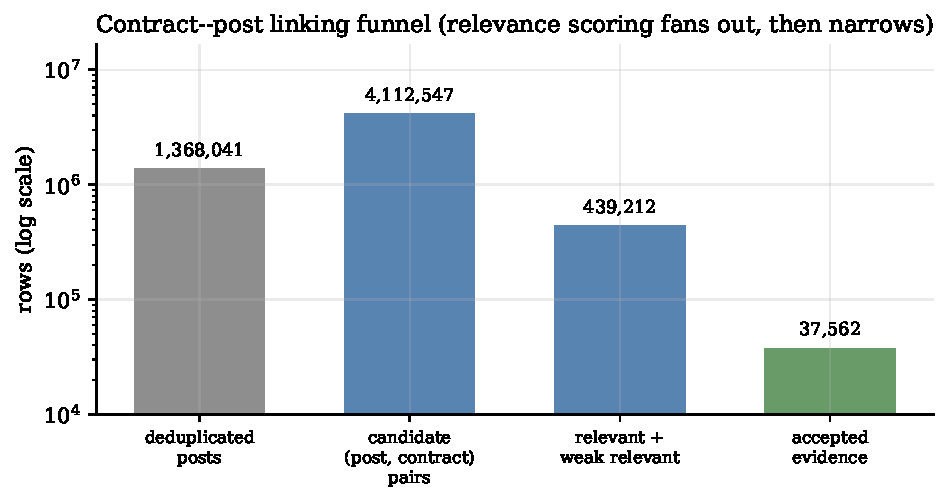
\includegraphics[width=0.92\linewidth]{fig_linking_funnel.pdf}
\caption{The linking funnel (log scale). Relevance scoring fans the corpus out into
\textbf{4{,}112{,}547} candidate (post, contract) pairs, of which only
\textbf{37{,}562} survive the acceptance policy as evidence. The largest losses are the
unrelated majority and the weak links below the confidence floor.}
\label{fig:funnel}
\end{figure}

\Cref{fig:confidence} explains why the funnel narrows so sharply: the bulk of scored
pairs sit in the $0.40$--$0.50$ confidence band, well below the $0.60$ acceptance
threshold. This conservative floor trades recall for precision --- a deliberate choice,
since downstream the cost of a spurious link (a post wrongly attributed to a contract)
is higher than the cost of a missed one.

\begin{figure}[H]
\centering
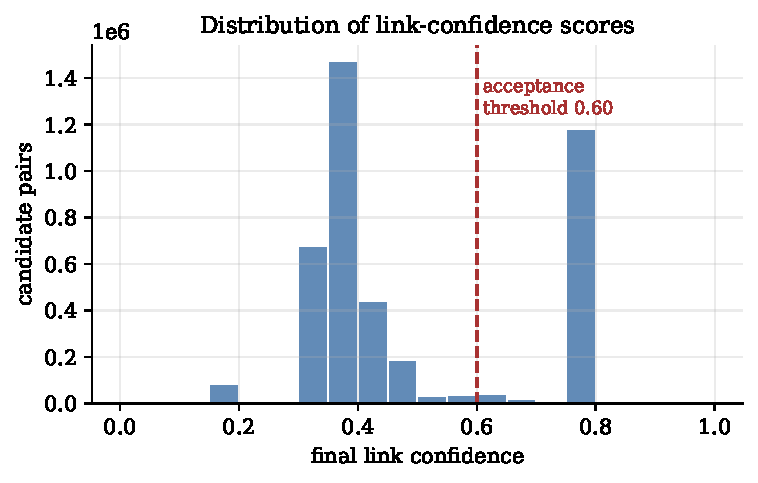
\includegraphics[width=0.74\linewidth]{fig_link_confidence.pdf}
\caption{Distribution of final link-confidence scores over all 4{,}112{,}547 candidates.
The dashed line marks the $0.60$ acceptance threshold for weakly-relevant links; most
candidates fall below it.}
\label{fig:confidence}
\end{figure}

\section{Coverage statistics}
The assignment asks for coverage statistics --- the fraction of contracts with at
least $k$ associated posts. \Cref{tab:link-labels} reports the relevance-label
breakdown, and \Cref{fig:coverage} the depth of accepted evidence per contract.
Accepted evidence reaches \textbf{147 of 300 contracts (49\%)}; 35~contracts have at
least 100 accepted links, while 153~have none. This uneven coverage is the central
data-quality story of the project and is dissected in
\Cref{ch:crossplatform,ch:limitations}.

\begin{table}[H]
\centering
\caption{Relevance labels over all 4{,}112{,}547 scored candidate pairs. Broad
retrieval makes \emph{unrelated} the majority label; the acceptance policy then keeps a
small, high-precision evidence set.}
\label{tab:link-labels}
\small
\begin{tabular}{@{}l r r@{}}
\toprule
\textbf{Relevance label} & \textbf{Pairs} & \textbf{Share}\\
\midrule
relevant         & 26{,}337      & 0.6\%\\
weakly\_relevant & 412{,}875     & 10.0\%\\
ambiguous        & 150{,}352     & 3.7\%\\
unrelated        & 3{,}522{,}983 & 85.7\%\\
\midrule
\textbf{Total scored} & \textbf{4{,}112{,}547} & 100\%\\
\addlinespace[2pt]
\textbf{Accepted as evidence} & \textbf{37{,}562} & 0.9\%\\
\bottomrule
\end{tabular}
\end{table}

\begin{figure}[H]
\centering
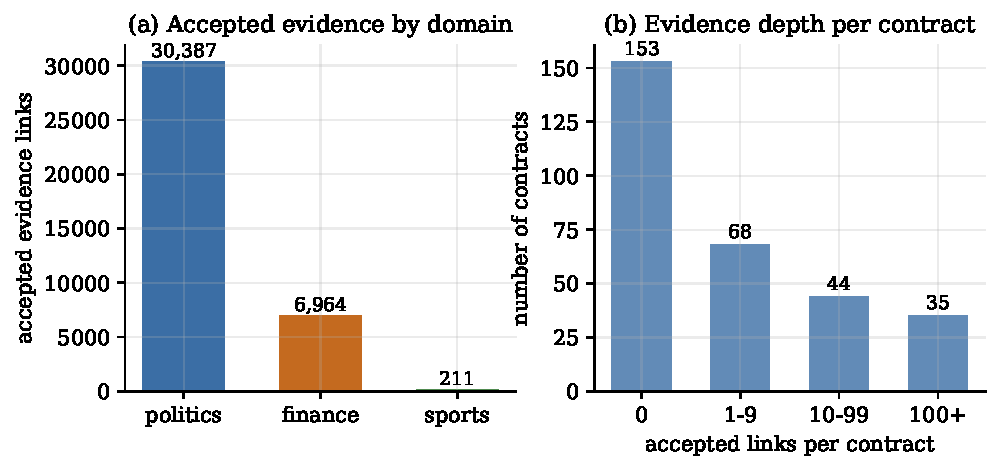
\includegraphics[width=\linewidth]{fig_evidence_coverage.pdf}
\caption{Evidence coverage. (a)~Accepted evidence is dominated by the politics domain
($30{,}387$ links) and almost absent for sports ($211$). (b)~Depth of accepted
evidence per contract: 153 contracts have no accepted evidence, 35 have $\geq 100$
links.}
\label{fig:coverage}
\end{figure}


%==============================================================================
\chapter{Text Preprocessing and NLP Enrichment}
\label{ch:nlp}

Enrichment turns raw post text into the structured fields required by the assignment
(hashtags, mentioned entities, language) and the analytical signals used later
(sentiment, topics, stance). To respect the data-safety convention of never rewriting
the ${\sim}300$\,MB raw corpus, all enrichment is written to \emph{derived tables}
keyed by \code{post\_id}, exactly like the linking and stance outputs. Every backend
degrades gracefully so the pipeline always runs offline, and the chosen backend is
recorded per row.

\section{Normalisation, language, hashtags, entities}
Text is lower-cased and stripped of control characters for matching while the original
is retained for display; timestamps are normalised to UTC (\Cref{ch:ingestion}).
\textbf{Language} is detected with \code{langdetect} when available, otherwise a
Cyrillic/stop-word heuristic; English dominates (1{,}118{,}413 enriched posts), followed
by Russian (105{,}395), reflecting the geopolitics channels. \textbf{Hashtags and
mentions} are extracted by deterministic regular expressions. \textbf{Named entities}
are extracted with spaCy~\cite{honnibal2017spacy} when installed, otherwise a
heuristic gazetteer-plus-capitalised-$n$-gram backend; the run reported here used the
heuristic backend over all \textbf{1{,}368{,}041} enriched posts. Its limitations
(channel handles and news boilerplate leaking in as pseudo-entities) are discussed in
\Cref{ch:discourse}.

\section{Sentiment analysis}
Sentiment is computed with \textbf{VADER}~\cite{hutto2014vader}, a rule-based model
tuned for social text (emoji, capitalisation, slang) and a sensible default that needs
no training data. Each post receives positive/neutral/negative proportions and a
\code{compound} score in $[-1,1]$, thresholded at $\pm 0.05$ into a label. A
transformer backend (\code{twitter-roberta}) is available as an opt-in upgrade. The
distribution of sentiment is analysed in \Cref{ch:discourse}; here we note only that
sentiment is a \emph{generic} polarity signal, deliberately distinct from stance.

\section{Topic modelling}
Topics are extracted with \textbf{Latent Dirichlet Allocation}~\cite{blei2003lda}
over \code{CountVectorizer} features (scikit-learn~\cite{pedregosa2011scikit}), run
over the \emph{linked} posts --- the discourse that actually concerns the contracts.
The vectoriser keeps the top \textbf{2{,}000} alphabetic terms (token pattern
\code{[a-zA-Z]\{2,\}}, unigrams), drops terms appearing in more than $60\%$ of documents
or in fewer than three, and removes both the standard English stop-word list and a
curated set of social/market boilerplate (e.g.\ ``http'', ``rt'', ``amp'', ticker
chatter). LDA is then fit with \textbf{ten topics}, the \code{"batch"} learning method,
\textbf{20} iterations, and a fixed \code{random\_state=42}; each topic is summarised by
its twelve highest-weight terms. We report ten topics as a deliberate, interpretable
granularity rather than tuning topic count by a coherence criterion --- the topics are
used qualitatively, to characterise \emph{what} the linked discourse is about, not as a
predictive feature. The resulting topics and their interpretation are presented in
\Cref{ch:discourse}.

\section{Outcome-aware stance}
\label{sec:stance}
Stance is the directional signal that feeds prediction, and it is computed
\emph{relative to each contract's outcomes}, not as generic polarity. For every
accepted \code{(contract, post)} link the stance module interprets the post against the
\textsc{Yes}/\textsc{No} proposition using outcome-specific cues, negation handling,
and uncertainty markers, emitting a label in \{\code{supports\_yes},
\code{supports\_no}, \code{neutral}, \code{ambiguous}, \code{insufficient\_context}\}
with a confidence. The deterministic heuristic labelled \textbf{35{,}679} post--outcome
rows across 140 contracts; \Cref{fig:stance} shows the distribution.

\begin{figure}[H]
\centering
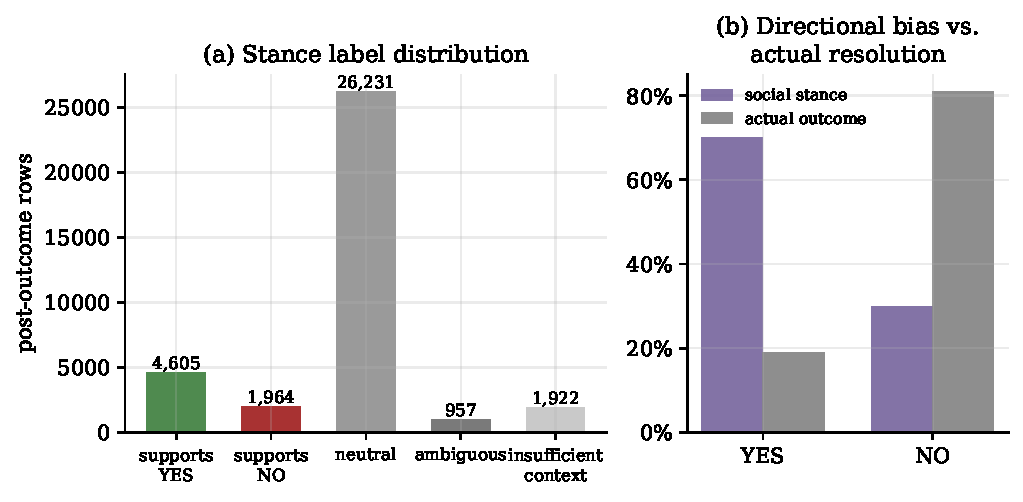
\includegraphics[width=\linewidth]{fig_stance.pdf}
\caption{Outcome-aware stance. (a)~Most rows are \code{neutral} (26{,}231); directional
rows split 4{,}605 \textsc{Yes} vs.\ 1{,}964 \textsc{No}. (b)~The social stance is
\textbf{2.3:1 biased towards \textsc{Yes}}, whereas the contracts actually resolve
\textbf{4.3:1 towards \textsc{No}} --- the optimism/hype mismatch that recurs
throughout the predictive analysis.}
\label{fig:stance}
\end{figure}

\begin{takeaway}
\textbf{Sentiment vs.\ stance.} Sentiment (VADER) measures the mood of the text;
stance measures its directional position on a contract's outcome. Both are computed,
but only stance feeds the forecast --- and stance already reveals a systematic
\textsc{Yes}-bias that foreshadows the predictive null result.
\end{takeaway}

%==============================================================================
%  PART 3 --- ANALYTICAL STUDY (Task 2)
%  Chapters: Descriptive (contracts) | Discourse | Signal-Market Correlation |
%            Cross-Platform | Dashboard
%==============================================================================

\chapter{Descriptive Analysis of Polymarket Contracts}
\label{ch:descriptive}

This chapter characterises the 300 contracts along the dimensions the assignment asks
for --- domain, duration, volume, and volatility --- and then studies how
market-implied probabilities evolve, and how informative they are of the final outcome
at different distances from resolution.

\section{Domain, duration, volume, and volatility}
\Cref{tab:descriptive} summarises the three thematic domains, and reveals that they are
qualitatively different objects despite the equal count.

\begin{table}[H]
\centering
\caption{Descriptive profile of the contracts by thematic domain
(medians; duration IQR in brackets).}
\label{tab:descriptive}
\small
\begin{tabular}{@{}l r r r r r@{}}
\toprule
\textbf{Domain} & \textbf{Contracts} & \textbf{Duration (d)} & \textbf{Volume (USD)} &
\textbf{YES-price vol.} & \textbf{\% YES}\\
\midrule
politics & 100 & 84 \,[28--181] & 25.5\,M & 0.070 & 33\%\\
finance  & 100 & 104 \,[31--134] & 20.8\,M & \textbf{0.114} & 20\%\\
sports   & 100 & \textbf{258} \,[249--272] & \textbf{41.6\,M} & \textbf{0.003} & 4\%\\
\midrule
\textbf{all} & 300 & 154 & 24.9\,M & 0.025 & 19\%\\
\bottomrule
\end{tabular}
\end{table}

\noindent Three patterns stand out (\Cref{fig:durvol,fig:volat}):
\begin{itemize}
  \item \textbf{Sports contracts are long-lived, high-volume long-shots.} They run for
  a whole season (median 258 days), attract the largest median volume, yet have the
  \emph{lowest} price volatility ($0.003$) and resolve \textsc{No} 96\% of the time ---
  they are mostly ``will team $X$ win the league?'' markets that sit near a stable, low
  probability for months and then resolve against the field.
  \item \textbf{Finance contracts are the most volatile} ($0.114$): crypto price-level
  bets (``Bitcoin above \$$X$'') swing as the underlying asset moves.
  \item \textbf{Politics contracts are the shortest and most balanced} in outcome
  (33\% \textsc{Yes}), consistent with sharp, event-driven questions.
\end{itemize}

\begin{figure}[H]
\centering
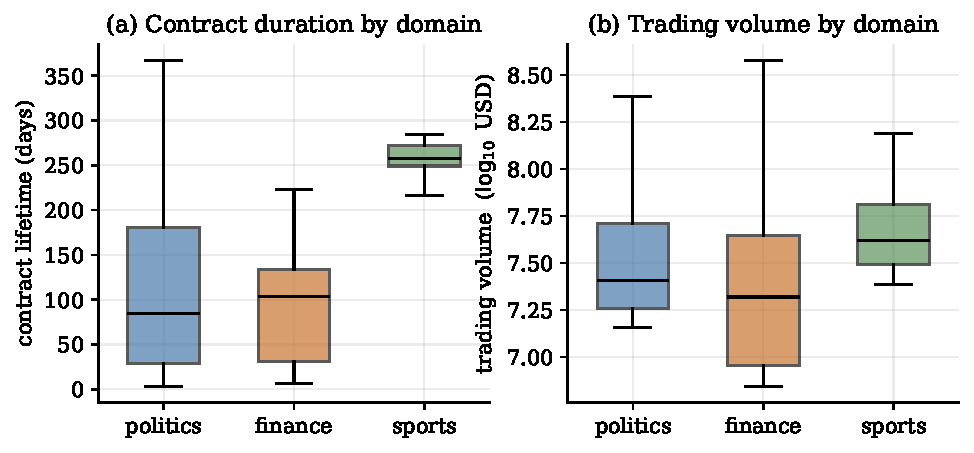
\includegraphics[width=\linewidth]{fig_duration_volume.pdf}
\caption{Contract lifetime (a) and trading volume (b) by domain. Sports contracts are
markedly longer-lived; volumes are large across the board (note the $\log_{10}$ scale).}
\label{fig:durvol}
\end{figure}

\begin{figure}[H]
\centering
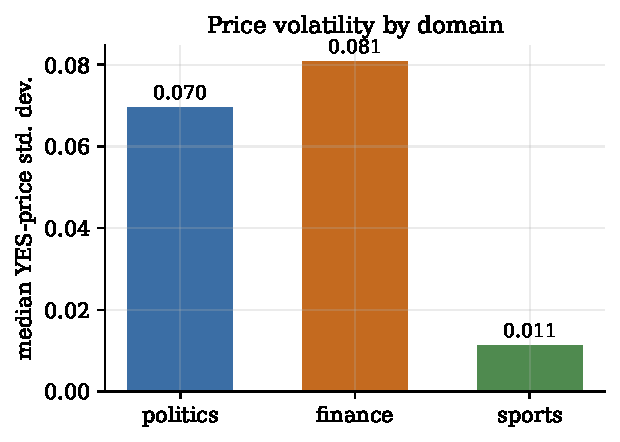
\includegraphics[width=0.56\linewidth]{fig_price_volatility.pdf}
\caption{Median volatility of the \textsc{Yes} price by domain. Finance is an order of
magnitude more volatile than sports.}
\label{fig:volat}
\end{figure}

\section{Are prices informative of the outcome?}
\label{sec:informative}
The central descriptive question is whether the market price is informative of the
final outcome, and how that informativeness depends on the distance to resolution. We
take, for each contract, the latest \textsc{Yes} price at least $h$ days before close,
treat it as a probabilistic forecast $\hat{p}=\Pr(\textsc{Yes})$, and score it against
the realised outcome with AUC and the Brier score
$\frac{1}{N}\sum_i (\hat{p}_i - y_i)^2$~\cite{brier1950verification}.
\Cref{fig:informative} shows the result.

\begin{figure}[H]
\centering
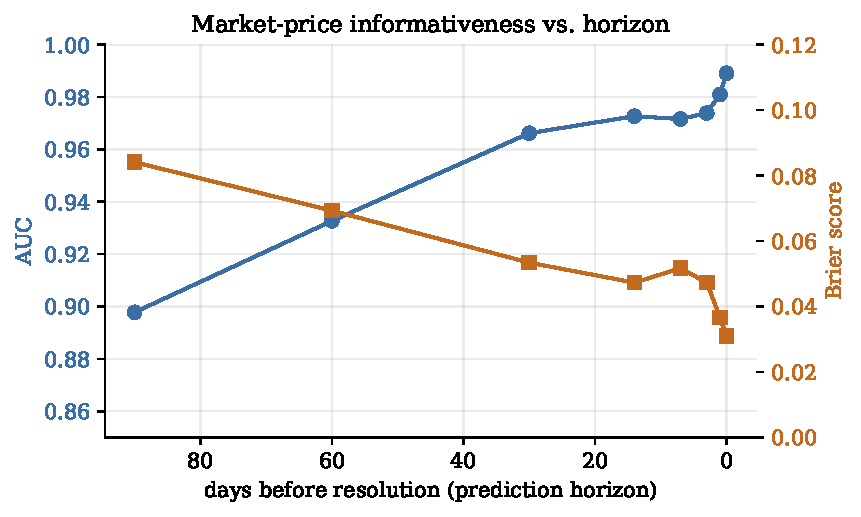
\includegraphics[width=0.72\linewidth]{fig_price_informativeness.pdf}
\caption{Market-price informativeness as a function of the prediction horizon (the
$x$-axis runs from 90 days before resolution, left, to the close, right). AUC rises
monotonically from $0.90$ to $0.99$ and the Brier score falls from $0.084$ to $0.031$
as resolution approaches.}
\label{fig:informative}
\end{figure}

\noindent The market is already a \emph{strong} forecaster three months out (AUC
$0.90$) and becomes near-perfect at the close (AUC $0.99$, Brier $0.031$). This is the
textbook behaviour of an efficient market resolving uncertainty over
time~\cite{wolfers2004prediction}, and it has a decisive consequence for the rest of
the report: \textbf{the bar any social signal must clear --- adding value on top of a
price that is already this informative --- is very high}. We return to this in
\Cref{ch:prediction}.

\begin{takeaway}
The market price alone separates \textsc{Yes} from \textsc{No} contracts with
AUC~$0.90$ three months before resolution and AUC~$0.99$ at the close. Informativeness
grows monotonically as the event nears.
\end{takeaway}


%==============================================================================
\chapter{Social-Media Discourse Analysis}
\label{ch:discourse}

We now characterise the discourse: its volume and timing, its sentiment, the entities
and topics that dominate it, and how these differ across platforms and domains
(Task~2.2).

\section{Volume, timing, and sources}
The corpus spans a decade of channel history but is concentrated in recent years, with
the analysis focused on the post-2024 window in which the studied contracts are active
(\Cref{fig:volume}). It is overwhelmingly a \textbf{Telegram} corpus
(98.6\%); Reddit contributes 16{,}254 posts (1.2\%) and X/Twitter a further 2{,}822
(0.2\%), a small but real third platform whose scale is capped by its anti-automation
defences (\Cref{sec:scope}). Volume is concentrated in a handful of large channels
(\Cref{fig:channels}): crypto exchanges and news aggregators (\code{CryptoComOfficial},
\code{cointelegraph}), macro/markets feeds (\code{zerohedge}, \code{FinancialJuice},
\code{WalterBloomberg}), and geopolitics/OSINT channels (\code{nexta\_live},
\code{ClashReport}, \code{intelslava}, \code{rybar}). This channel mix is the single
most important fact about the corpus: \textbf{it is a crypto/macro/geopolitics corpus,
with essentially no sports coverage} --- a mismatch we quantify in
\Cref{ch:crossplatform}.

\begin{figure}[H]
\centering
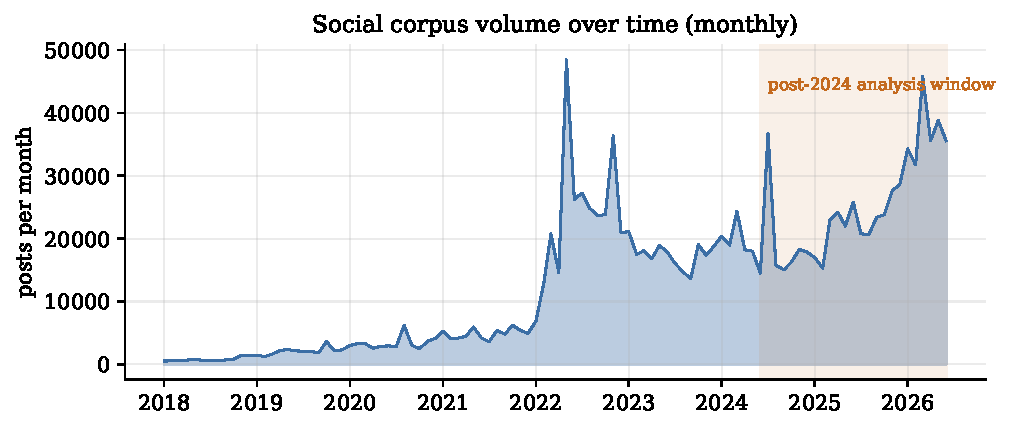
\includegraphics[width=\linewidth]{fig_social_volume.pdf}
\caption{Monthly volume of the social corpus. Activity accelerates through 2024--2026;
the shaded region marks the analysis window in which the studied contracts are live.}
\label{fig:volume}
\end{figure}

\begin{figure}[H]
\centering
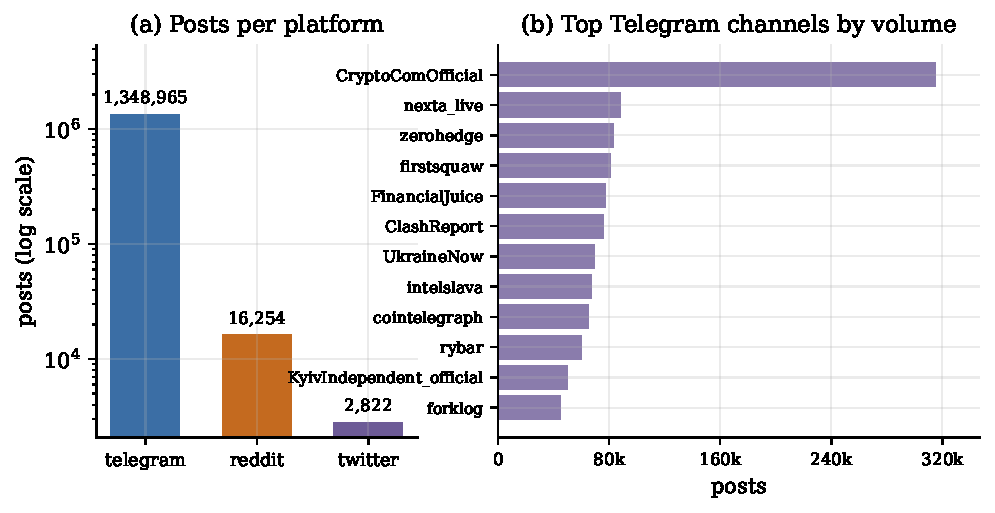
\includegraphics[width=\linewidth]{fig_corpus_platform_channels.pdf}
\caption{(a) Posts per platform (log scale): Telegram dominates. (b) The largest
Telegram channels are crypto, macro, and geopolitics sources.}
\label{fig:channels}
\end{figure}

\section{Sentiment}
Sentiment, computed with VADER (\Cref{ch:nlp}), is close to balanced but slightly
positive on aggregate (mean compound $+0.006$): \textbf{48\% neutral, 28\% positive,
24\% negative} (\Cref{fig:sentiment}). The neutral mass is expected for a corpus heavy
in news-wire and OSINT reporting (``\textsc{Breaking}: \dots''), whose register is
factual. The platform breakdown is similar on Telegram and Reddit, so sentiment does
not, by itself, distinguish the two sources.

\begin{figure}[H]
\centering
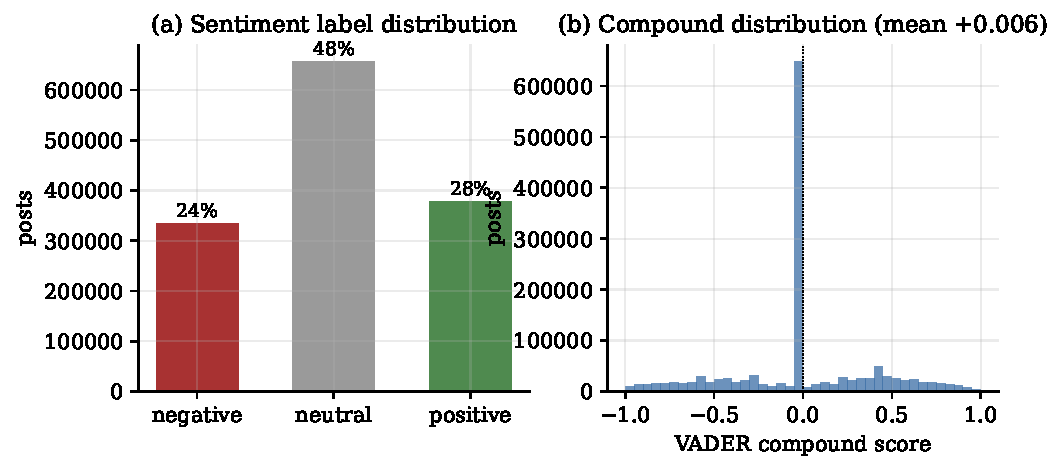
\includegraphics[width=\linewidth]{fig_sentiment.pdf}
\caption{(a) Sentiment-label distribution over 1{,}368{,}041 enriched posts. (b) The VADER
compound score is centred near zero with a slight positive tilt.}
\label{fig:sentiment}
\end{figure}

\section{Named entities}
The most frequent entities (\Cref{fig:entities}) trace the corpus's preoccupations:
\emph{Trump}, the \emph{US}, \emph{Ukraine}, \emph{Iran}, \emph{Russia}, \emph{Israel},
\emph{Gaza}, the \emph{Fed}, \emph{China}, and \emph{Bitcoin}. The list confirms a
politics, geopolitics, macro, and crypto corpus, and the near-total absence of sports
entities. It also exposes an honest limitation of the heuristic NER backend: a few
high-frequency ``entities'' are in fact channel handles or news boilerplate (e.g.\
broadcast-footer tokens, app names such as \emph{WhatsApp} and \emph{Viber}, and markers
like \emph{Breaking} or \emph{Just In}). We filter the most obvious of these from
\Cref{fig:entities}; a
production system would use the spaCy backend (available but not used at scale here) and
a stop-entity list. The artefact does not affect the predictive results, which depend on
stance, not on raw entity counts.

\begin{figure}[H]
\centering
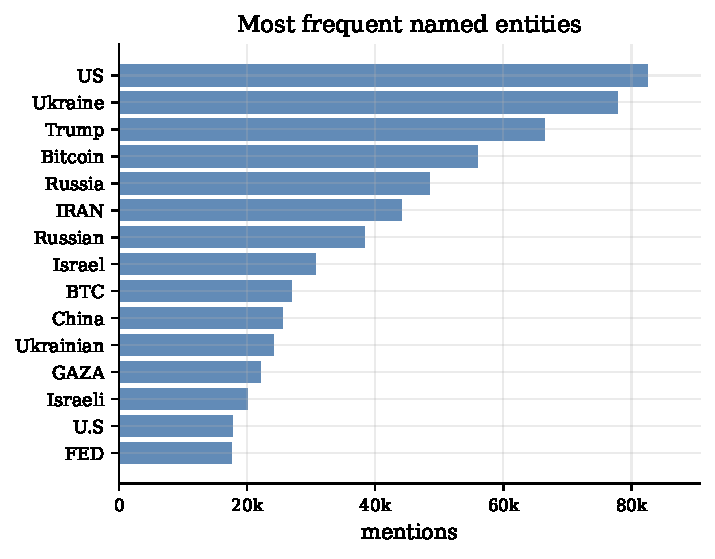
\includegraphics[width=0.66\linewidth]{fig_entities.pdf}
\caption{Most frequent named entities (obvious channel/app/boilerplate tokens removed).
The corpus is dominated by geopolitics, macro, and crypto references.}
\label{fig:entities}
\end{figure}

\section{Topics}
Latent Dirichlet Allocation over the linked posts yields ten coherent topics
(\Cref{fig:topics,tab:topics}). They partition cleanly into \emph{geopolitics}
(Iran--Israel strikes, Iran nuclear talks, Trump and Ukraine, the Iranian regime),
\emph{macro} (Fed, rates, inflation), and \emph{crypto} (Bitcoin, Ethereum, and
trading groups). No topic is about sports. The topic structure thus mirrors the
entity and channel analyses: three things the corpus talks about a great deal, and one
of the three required domains it barely mentions.

\begin{figure}[H]
\centering
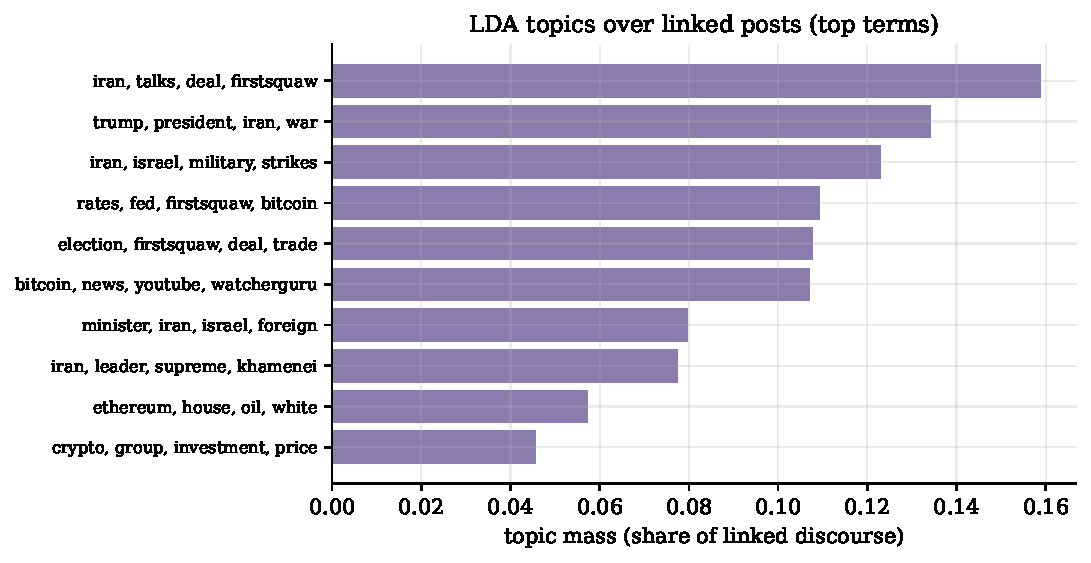
\includegraphics[width=0.74\linewidth]{fig_topics.pdf}
\caption{LDA topic mass over the linked discourse. Geopolitics, macro, and crypto
topics dominate; sports is absent.}
\label{fig:topics}
\end{figure}

\begin{table}[H]
\centering
\caption{The ten LDA topics over linked posts, by mass, with their leading terms.}
\label{tab:topics}
\small
\begin{tabularx}{\linewidth}{@{}r l X@{}}
\toprule
\textbf{Mass} & \textbf{Theme} & \textbf{Top terms}\\
\midrule
0.159 & Iran nuclear talks & iran, talks, deal, trump, russia, nuclear, ukraine\\
0.134 & Trump / war / Ukraine & trump, president, iran, war, ukraine, russia, ceasefire\\
0.123 & Iran--Israel strikes & iran, israel, military, strikes, iranian, missile, regime\\
0.109 & Fed / rates & rates, fed, inflation, policy, rate, hold, cut\\
0.108 & Elections / trade & election, deal, trade, rates, fed, president, japan\\
0.107 & Bitcoin / crypto news & bitcoin, news, btc, crypto, ethereum, saylor, bank\\
0.080 & Diplomacy / ministers & minister, iran, israel, foreign, prime, rubio, security\\
0.077 & Iran supreme leader & iran, leader, supreme, khamenei, iranian, killed\\
0.057 & Ethereum / oil / WH & ethereum, house, oil, white, buterin, vitalik\\
0.046 & Crypto trading groups & crypto, group, investment, price, sell, buy, discussion\\
\bottomrule
\end{tabularx}
\end{table}


%==============================================================================
\chapter{Signal--Market Correlation}
\label{ch:correlation}

This chapter studies the temporal relationship between the social signal and the market
price (Task~2.3): does social activity precede, coincide with, or follow price moves,
and is the direction of social stance aligned with the direction of price change?

\section{Constructing the social signal}
\label{sec:spi-signal}
To compare social discourse against price on the same axis, we condense the accepted,
directional evidence into a per-day social estimate of $\Pr(\textsc{Yes})$. Let
$w^{+}_t$ and $w^{-}_t$ be the day-$t$ \textsc{Yes}/\textsc{No} evidence weights, where
each stance contributes $\text{confidence}\times(1+\log(1+\text{engagement}))$, capped
at $4.0$ per post and at $3.0$ per source per market-day so that no single author or
channel dominates a market-day (source diversity), and the
daily totals are EWMA-smoothed with a 3-day half-life. The social signal and its
strength are then
\begin{equation}
s_t \;=\; \frac{w^{+}_t + \tfrac{\kappa}{2}}{w^{+}_t + w^{-}_t + \kappa},
\qquad
\sigma_t \;=\; \frac{w^{+}_t + w^{-}_t}{w^{+}_t + w^{-}_t + \kappa}\;\in[0,1),
\label{eq:signal}
\end{equation}
a Laplace-smoothed estimate anchored at $0.5$ with pseudo-count $\kappa=1.5$
(implemented as a per-side $\alpha=0.75$): on thin-evidence days $\sigma_t\!\approx\!0$
and $s_t\!\approx\!0.5$, so the signal does not spike on noise. We treat the social line
as meaningful only where $\sigma_t$ is well above zero.

\section{Do social spikes lead, coincide with, or follow price moves?}
We answer this quantitatively. On days with meaningful evidence ($\sigma_t>0.2$;
$1{,}848$ contract-days over $66$ contracts), the pooled Pearson correlation between
$s_t$ and the market probability is only $\mathbf{0.05}$, and the median per-contract
correlation is $0.09$ (\Cref{fig:leadlag}b) --- weak and scattered around zero. To test
\emph{direction}, we cross-correlate daily \emph{changes}, $\Delta s_t$ against
$\Delta p_{t+k}$, for lags $k\in[-7,7]$ pooled over the well-covered contracts
(\Cref{fig:leadlag}a): a positive lag $k$ means the price moves \emph{after} the social
signal, i.e.\ social would be \emph{leading}. The profile is essentially flat --- every
lag stays within $|r|<0.04$ --- and the only mild peak sits at lag $0$ (coincident), with
\textbf{no positive-lead peak}. There is therefore no horizon at which social changes
systematically precede price changes: the little structure that exists is coincident at
best, consistent with discourse \emph{reacting} to, rather than anticipating, the events
the market prices.

\begin{figure}[H]
\centering
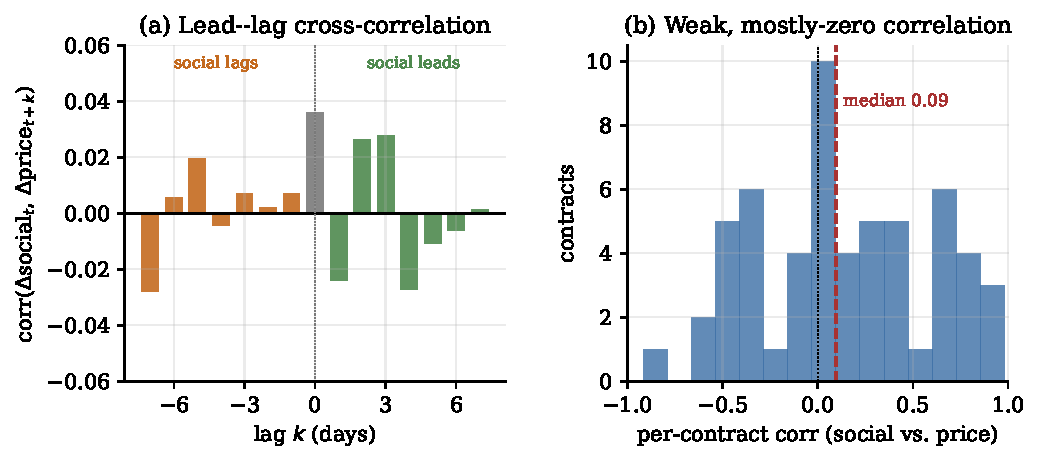
\includegraphics[width=\linewidth]{fig_leadlag.pdf}
\caption{Social signal versus price, quantitatively. (a)~Lead--lag cross-correlation of
daily changes: a positive lag ($k>0$) would mean social \emph{leads} the price, yet every
lag stays within $|r|<0.04$ and the only mild peak is at lag $0$ (coincident) --- there is
no positive-lead peak. (b)~Distribution of per-contract social--price correlations: weak
and centred near zero (median $0.09$). Together they show the social signal neither leads
nor meaningfully tracks the market price.}
\label{fig:leadlag}
\end{figure}

\section{Is the direction of stance aligned with the outcome?}
Aggregating stance into a per-contract direction (\Cref{eq:signal} at the final
pre-close cut), the directional agreement between the social signal and the realised
outcome is only $\mathbf{0.21}$ --- worse than a coin flip --- and the correlation
between the aggregate stance balance and the outcome is $-0.015$ (essentially zero). The
reason is the optimism mismatch already visible in \Cref{fig:stance}: among the
72 contracts on which social pressure points \textsc{Yes}, only 14 actually resolved
\textsc{Yes} (\Cref{fig:hype}). Social discourse is systematically biased towards the
exciting \textsc{Yes} outcome, while the contracts overwhelmingly resolve \textsc{No}.

\begin{figure}[H]
\centering
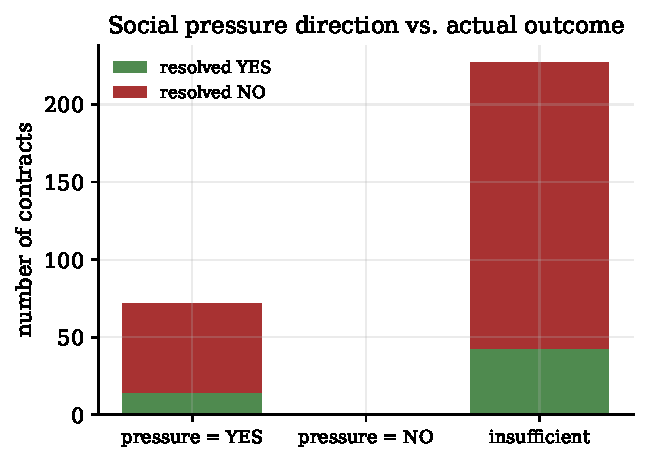
\includegraphics[width=0.56\linewidth]{fig_hype_mismatch.pdf}
\caption{Social-pressure direction versus actual outcome. Where social pressure says
\textsc{Yes} (72 contracts), the market still resolves \textsc{No} 58 times; the social
direction is anti-correlated with reality.}
\label{fig:hype}
\end{figure}

\begin{takeaway}
Social activity neither leads nor strongly coincides with price (pooled correlation
$0.05$, flat lead--lag profile), and its \emph{direction} is anti-aligned with outcomes
(agreement $0.21$). The discourse is reactive and optimism-biased.
\end{takeaway}


%==============================================================================
\chapter{Cross-Platform Comparison}
\label{ch:crossplatform}

Task~2.4 asks three concrete questions: do the platforms carry \emph{complementary} or
\emph{redundant} signals; are there contracts for which one platform is substantially
more informative than the others; and what distinguishes those cases. This chapter
answers each over all three collected platforms (Telegram, Reddit, and X/Twitter),
with Telegram supplying the overwhelming majority of posts (\Cref{sec:scope}). The
cross-platform layer reads from \code{cross\_platform\_comparison.parquet} (one row
per contract that carries social discourse) and its per-domain roll-up
\code{cross\_platform\_summary.parquet}.

\section{How many platforms cover each contract?}
\label{sec:xplat-coverage}
Of the 300 contracts, \textbf{232 carry at least one linked social post}, and
\textbf{181 of those are multi-platform} --- discussed on at least two of Telegram,
Reddit, and X/Twitter within the analysis window, with \textbf{114 carrying all three}.
\Cref{tab:xplat} breaks the 232 down by domain, and \Cref{fig:xplat} visualises it.

\begin{table}[H]
\centering
\caption[Per-domain platform coverage]{Platform coverage by domain over the 232 contracts
that carry social discourse. \emph{Single} = one platform present;
\emph{multi} = at least two platforms present; \emph{compl.} = contracts the
cross-platform analysis flags as genuinely \emph{complementary} (a minority platform
contributes non-trivially rather than echoing the majority).}
\label{tab:xplat}
\small
\begin{tabular}{@{}l r r r r@{}}
\toprule
\textbf{Domain} & \textbf{With social} & \textbf{Single-platform} & \textbf{Multi-platform} & \textbf{Complementary}\\
\midrule
politics & 85  & 21 & 64  & 1\\
finance  & 58  & 10 & 48  & 0\\
sports   & 89  & 20 & 69  & \textbf{28}\\
\midrule
\textbf{total} & \textbf{232} & 51 & 181 & 29\\
\bottomrule
\end{tabular}
\end{table}

\begin{figure}[H]
\centering
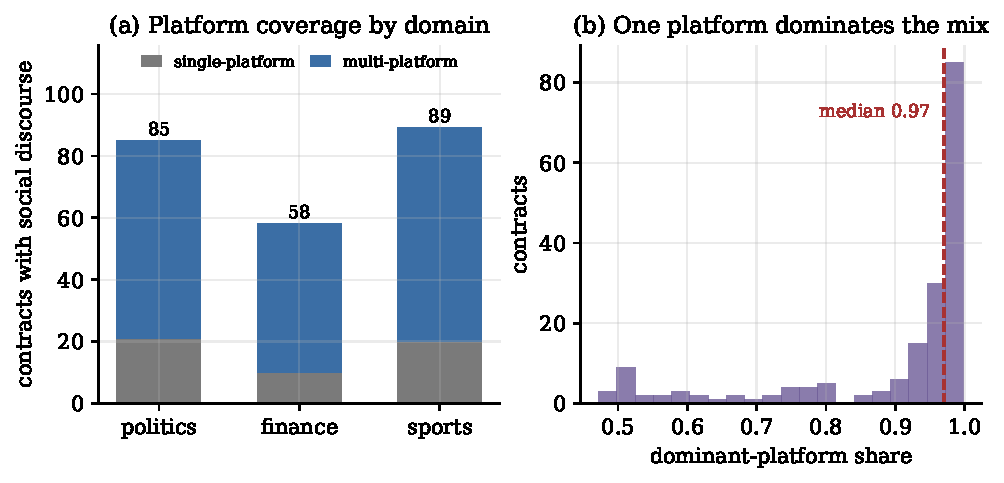
\includegraphics[width=\linewidth]{fig_cross_platform.pdf}
\caption{Cross-platform coverage. (a)~Single- vs multi-platform contracts by domain:
most covered contracts appear on both platforms. (b)~Distribution of the
\emph{dominant-platform share} over multi-platform contracts --- Telegram supplies the
overwhelming majority of posts even when Reddit is also present, so the two signals are
mostly \textbf{redundant rather than complementary}.}
\label{fig:xplat}
\end{figure}

\section{Redundant or complementary?}
On the 181 multi-platform contracts the \emph{dominant platform} (Telegram in almost
every case) accounts for a median share of ${\sim}\mathbf{0.97}$ of the posts: when
several platforms speak about a contract, they say the same thing and Telegram says far
more of it. By the standard meaning of the question, the signals are therefore
\textbf{redundant, not complementary} --- adding Reddit or X to Telegram rarely changes
the per-contract social estimate. The lone exception is \textbf{sports}: 28 sports
contracts are flagged complementary, precisely because Telegram barely covers sports
(\Cref{sec:xplat-mismatch}), so what little signal exists there comes disproportionately
from Reddit. This is the one corner of the dataset where a second platform measurably
adds coverage.

\section{Where is one platform substantially more informative?}
The per-contract view identifies the cases the assignment asks for. For
\emph{geopolitics and macro} contracts --- US--Iran, Russia--Ukraine, the Fed --- Telegram
is overwhelmingly the more informative platform, contributing thousands of posts where
Reddit contributes tens. For the handful of \emph{sports} contracts that are covered at
all, Reddit is relatively (though still thinly) the more informative source. No contract
in the snapshot is substantially better covered by Reddit than Telegram in absolute
terms; that asymmetry is a property of the collected channel mix, and the cross-platform
table is the artefact that would surface the reverse cases under a broader collection.

\section{A genuine three-platform comparison}
Because every platform normalises to the same \code{SocialPostRecord} and the
cross-platform analysis keys only on \code{platform}, all three sources enter
\Cref{tab:xplat,fig:xplat} uniformly: \textbf{114 of the 232 covered contracts carry
posts from all three platforms}. X/Twitter's contribution is small in volume
(\Cref{sec:scope}), so Telegram still dominates the per-contract mix, but the comparison
is genuinely three-platform rather than a two-platform result with a placeholder column.
Broadening the X or Reddit pass would repopulate this chapter with no code change ---
re-running \code{polysignal analytics run} followed by the figure regeneration is all
that is required.

\section{The channel--market mismatch}
\label{sec:xplat-mismatch}
The more consequential cross-cutting comparison is not between platforms but between
the \emph{topics} the channels discuss and the \emph{domains} of the contracts.
\Cref{tab:mismatch} lays the mismatch bare: politics contracts absorb 81\% of all
accepted evidence, finance most of the rest, and \textbf{sports almost none} (211 links
across 100 contracts). The channels are crypto/macro/geopolitics sources; they simply do
not talk about who will win the Premier League.

\begin{table}[H]
\centering
\caption{Accepted evidence by domain, against the equal contract counts. Social evidence
is concentrated where the channels' topics lie, not where the contracts are.}
\label{tab:mismatch}
\small
\begin{tabular}{@{}l r r r@{}}
\toprule
\textbf{Domain} & \textbf{Contracts} & \textbf{Accepted links} & \textbf{Share of evidence}\\
\midrule
politics & 100 & 30{,}387 & 80.9\%\\
finance  & 100 & 6{,}964  & 18.5\%\\
sports   & 100 & 211      & 0.6\%\\
\midrule
\textbf{total} & 300 & 37{,}562 & 100\%\\
\bottomrule
\end{tabular}
\end{table}

\noindent The contracts for which social discourse is by far the most informative are
therefore the \emph{geopolitics} ones --- US--Iran, Russia--Ukraine, Israel--Iran ---
which attract thousands of accepted links each, while crypto price-level and Fed-rate
contracts attract hundreds and sports contracts attract a handful. This is the key
qualitative finding of the cross-cutting analysis, and it directly explains the
predictive results of Part~IV: the social signal is dense and usable for one slice of
the market and absent for another.


%==============================================================================
\chapter{Interactive Dashboard}
\label{ch:dashboard}

All results are exposed through a custom interactive \textbf{React}~\cite{react}
single-page application (designed and built with Claude's design tooling, \emph{not} the
suggested Streamlit~\cite{streamlit2023} default, to obtain a more polished and
customisable interface). It is served on a single local origin by a small, zero-dependency
Python API (\code{scripts/serve\_app.py}, launched by \code{run\_app.cmd}) that materialises
the exact persisted artefacts behind this report into the \code{window.PS\_DATA} contract:
the app needs \emph{no internet, no CORS, and no build step}, never recomputes features,
retrains models, or calls an external service, so a live demo is deterministic and fast.
The application is the deliverable shown live during the oral discussion.

\section{Views}
The app is organised as two linked views plus a persistent customisation panel
(\Cref{tab:dashboard}). It opens on the \emph{Market Universe}; selecting any contract
drills into the \emph{Market Detail}.

\begin{table}[H]
\centering
\caption{The React dashboard: views, the panels they contain, and the Task-2 requirement
each satisfies.}
\label{tab:dashboard}
\small
\begin{tabularx}{\linewidth}{@{}l X@{}}
\toprule
\textbf{View / panel} & \textbf{What it shows}\\
\midrule
\textbf{Market Universe} & browse all 300 contracts as a card grid; filter by \emph{domain} (macro, politics, crypto, AI, sports, culture) and \emph{status} (active, closing, resolved); each card sparklines price vs.\ social signal\\
\textbf{Market Detail} & opens on the per-contract \emph{dual-line chart}: market $\Pr(\textsc{Yes})$ vs.\ the smoothed social signal (\Cref{eq:signal}), with event markers\\
\quad Social panel        & post volume, sentiment split, and the stance distribution for the contract\\
\quad Scorecard / Divergence & headline outcome, resolution date, and where social pressure \emph{diverges} from the price\\
\quad Cross-platform      & per-platform post mix for the contract (\Cref{ch:crossplatform})\\
\quad Evidence inspector  & individual linked posts with stance tag, sentiment, entities, engagement, and a ``why linked'' rationale\\
\quad Narrative graph      & the contract's neighbourhood in the Neo4j knowledge graph\\
\textbf{Tweaks panel}     & live customization: accent theme, layout density, chart style (pressure/area), and signal thresholds\\
\bottomrule
\end{tabularx}
\end{table}

\section{Design rationale}
The dashboard is designed directly against the five graded dashboard axes.
\emph{Priority}: it opens on the Universe and one click reaches the dual-line
price-vs-social chart --- the project's central comparison --- so the main idea is never
more than a click away. \emph{Accuracy}: every panel reads the exact persisted artefact
behind the corresponding number in this report, and thin-evidence contracts are flagged
rather than smoothed (the social line is drawn only where $\sigma_t$ is meaningful, per
\Cref{eq:signal}). \emph{Conciseness}: each panel answers one question and the card grid
compresses 300 contracts into a scannable overview. \emph{Usability}: domain/status
filters, sparkline cards, and a single-contract drill-down make navigation immediate.
\emph{Customization}: the Tweaks panel lets the user re-theme, re-densify, switch chart
styles, and re-threshold the signal live. The explicit browsing requirements of Task~2
--- browse by domain, resolution date and outcome; visualise price alongside social
activity; explore sentiment and engagement distributions; and inspect individual linked
posts with their metadata and extracted features --- are each served by one of the panels
above.

\paragraph{Reconciling the dashboard counts with the report.} Two deliberate display
choices make some headline counts differ between the live app and the figures in this
report, and we state them explicitly so the two artefacts are seen to agree. First, the
app renders the \textbf{295} contracts that pass its display guards --- a handful of
finance contracts whose only candidate links are off-subject, or whose price series is
degenerate, are held out of the \emph{demo} so no misleading card is ever shown --- while
the full \textbf{300}-contract dataset and \emph{every} analytic in this report use the
complete set. Second, the app's ``with-evidence'' badge uses a deliberately stricter
\emph{on-subject, directional} bar (\textbf{66} contracts) than the linking-layer coverage
quoted in \Cref{ch:linking} (\textbf{134} contracts with $\geq\!1$ accepted link), so that
a social card is drawn only where the evidence is genuinely informative. The two views are
consistent: they report coverage at different points of the same acceptance funnel
(\Cref{fig:funnel}), conservatively by design.

%==============================================================================
%  PART 4 --- PREDICTION & CONCLUSIONS (Task 3)
%  Chapters: Outcome Prediction | Discussion | Limitations & Future Work |
%            Conclusions
%==============================================================================

\chapter{Outcome Prediction from Social Features}
\label{ch:prediction}

This chapter undertakes the optional Task~3: it engineers social features, trains
forecasting models under a leakage-controlled, temporally honest protocol, and asks
directly whether social discourse improves on the market price. The answer is a clear
\emph{no}, and the value of the chapter is in establishing that answer rigorously, with
an ablation that isolates exactly the incremental contribution of the social signal.

\section{Feature engineering: the Task-3 feature matrix}
\label{sec:spi-features}
Task~3 starts from a single feature matrix with one row per resolved contract
(\code{task3\_\allowbreak feature\_\allowbreak matrix.parquet}, $300$ rows), assembled through the same
leakage-safe evaluation join used by the backtest. It realises all four feature families suggested by the
assignment, each computed strictly from \emph{pre-close, accepted} evidence:
\begin{description}[leftmargin=1.4em,style=nextline]
  \item[Volume.] Total accepted posts, posting growth rate (late-vs-early log ratio over
  the contract lifetime), unique authors and channels, and active days. The comments
  count is an honest zero, as per-comment text is collected only as a bounded sample.
  \item[Engagement.] Aggregate, mean, max and log-total engagement, plus a
  high-vs-low-engagement ratio relative to the corpus median.
  \item[Sentiment.] Mean and variance of VADER compound sentiment, the positive /
  negative / neutral fractions, and an early-vs-late sentiment trend.
  \item[Linguistic.] A per-contract text document over the accepted post text, turned
  into a TF--IDF representation reduced to $16$ latent dimensions by truncated SVD.
  Crucially this vectoriser is re-fit \emph{inside each training fold}, so the linguistic
  representation never leaks across the temporal split.
\end{description}
On top of these we carry the interpretable per-market \emph{Social Pressure Index} (SPI)
features (\Cref{tab:features}), which condense the stance-labelled evidence into a
compact, engagement-weighted directional signal, and the market arm contributes the
latest valid pre-close \textsc{Yes} price as its single predictor. \Cref{tab:features}
lists the SPI subset; the full matrix spans all four categories above.

\begin{table}[H]
\centering
\caption[The eight social features (SPI whitelist)]{The eight social features (the SPI
whitelist) and the assignment category each realises. Every feature is computed only
from pre-close, accepted evidence.}
\label{tab:features}
\small
\begin{tabularx}{\linewidth}{@{}l l X@{}}
\toprule
\textbf{Feature} & \textbf{Category} & \textbf{Definition}\\
\midrule
\code{stance\_balance}        & stance     & net directional lean $(n_{\textsc{y}}-n_{\textsc{n}})/(n_{\textsc{y}}+n_{\textsc{n}})$\\
\code{pressure\_strength}     & stance     & magnitude of the net (engagement-weighted) directional pressure\\
\code{temporal\_decay\_pressure} & temporal & net pressure weighted towards evidence near the close (recency)\\
\code{pressure\_acceleration} & temporal   & change in pressure between the early and late windows\\
\code{evidence\_quality\_score} & quality  & mean link/stance confidence of the accepted evidence\\
\code{source\_diversity\_score} & volume   & channel/author entropy (anti-spam source spread)\\
\code{accepted\_evidence\_ratio} & volume  & accepted links / scored candidates for the contract\\
\code{engagement\_log\_total}  & engagement & $\log(1+\text{total engagement})$ over accepted posts\\
\bottomrule
\end{tabularx}
\end{table}

\section{Models and evaluation protocol}
We evaluate three nested feature sets in increasing order of the information they use ---
\textbf{market-only} (the pre-close price), \textbf{social-only} (the full
volume\,+\,\allowbreak engagement\,+\,\allowbreak sentiment\,+\,\allowbreak linguistic\,+\,\allowbreak SPI matrix), and \textbf{market +
social} (both) --- against a Laplace-smoothed base-rate baseline. On every feature set we
train \textbf{four model families}: a regularised logistic regression, a Platt-calibrated
linear SVM, Gaussian naive Bayes, and a gradient-boosting ensemble (all class-balanced,
seed 42). Holding the model fixed and varying the feature set turns this $4\times3$ grid
into a full \emph{ablation} that isolates the incremental contribution of the social
signal across model families.

\noindent Because contracts are intrinsically ordered in time, we score them under an
\textbf{expanding-window temporal cross-validation} that respects chronology and forbids
leakage: contracts are sorted by close date and partitioned into five contiguous blocks;
fold $i$ trains on blocks $0..i$ and is scored on block $i{+}1$, so every prediction is
issued by a model trained only on \emph{earlier}-resolving contracts. This yields $250$
strictly out-of-fold predictions ($5$ folds $\times 50$). The leakage controls are
explicit and auditable: the feature table is rejected if it contains any
target/outcome/resolution column; labels are joined only after the social features pass
validation; the linguistic TF--IDF/SVD is re-fit per training fold; the market
probability is strictly pre-close; and settled post-resolution prices are never used.

\noindent The assignment's required metrics are \textbf{accuracy}, \textbf{macro-F1}, and
\textbf{AUC-ROC}; we add the Brier score~\cite{brier1950verification} and Expected
Calibration Error (ECE). Macro-F1 --- the unweighted mean of the two per-class F1 scores
--- is the headline metric here, because under the $57{:}243$ \textsc{Yes}{:}\textsc{No}
class imbalance a model that always predicts \textsc{No} already reaches $0.81$ accuracy:
\begin{gather}
\text{macro-F1}=\tfrac{1}{2}\big(\mathrm{F1}_{\textsc{Yes}}+\mathrm{F1}_{\textsc{No}}\big),
\qquad
\text{Brier}=\tfrac{1}{N}\!\sum_i (\hat p_i-y_i)^2,\\[2pt]
\text{ECE}=\!\sum_b \tfrac{n_b}{N}\,|\mathrm{acc}_b-\mathrm{conf}_b|.
\end{gather}

\noindent For full reproducibility, \Cref{tab:hyperparams} pins the exact configuration of
every model family. All estimators are class-balanced and share a fixed seed
($\code{random\_state}=42$); the linear SVM is wrapped in a sigmoid (Platt) calibrator so
that it, too, emits probabilities for the Brier/ECE/AUC computations. Two estimators
(Gaussian naive Bayes and gradient boosting) use the scikit-learn defaults deliberately:
with only $250$ out-of-fold points, tuning their many knobs would invite overfitting to
the evaluation, so we fix sensible defaults and let the \emph{feature set}, not
hyperparameter search, carry the comparison.

\begin{table}[H]
\centering
\caption[Model hyperparameters]{Exact model configuration (scikit-learn). All families
use \code{class\_weight="balanced"} and \code{random\_state=42}. ``default'' means the
scikit-learn default is used unchanged, by design.}
\label{tab:hyperparams}
\small
\begin{tabularx}{\linewidth}{@{}l X@{}}
\toprule
\textbf{Family} & \textbf{Configuration}\\
\midrule
Logistic regression & \code{C=0.5}, \code{solver="liblinear"} (L2 penalty), \code{max\_iter=1000}\\
Linear SVM          & \code{LinearSVC(C=0.5, max\_iter=5000)} wrapped in \code{CalibratedClassifierCV(method="sigmoid", cv=3)}\\
Gaussian naive Bayes & defaults (no smoothing override)\\
Gradient boosting   & defaults ($100$ stages, \code{max\_depth=3}, \code{learning\_rate=0.1})\\
\midrule
Linguistic features & \code{TfidfVectorizer} ($\le\!2000$ features, unigrams) $\to$ \code{TruncatedSVD($16$)}, re-fit \emph{per training fold}\\
Cross-validation    & expanding window, $5$ contiguous folds by close date\\
\bottomrule
\end{tabularx}
\end{table}

\section{Results: temporal-CV ablation}
\label{sec:results}
\Cref{tab:task3} and \Cref{fig:task3} report the primary result. Across all four model
families the \textbf{market arm is a strong forecaster} (macro-F1 $0.90$--$0.93$, AUC
$0.93$--$0.95$), while the \textbf{social-only arm collapses to near chance} (macro-F1
$0.47$--$0.51$, AUC $0.50$--$0.56$, barely above the $0.446$/$0.510$ base-rate baseline).
Combining the two never beats the market arm: the best combined configuration
(linear SVM, macro-F1 $0.933$) merely \emph{ties} the best market-only configuration
(macro-F1 $0.933$), and for naive Bayes the social features actively \emph{hurt}
(macro-F1 $0.918\!\to\!0.655$). The result is robust to the choice of model family.

\begin{table}[H]
\centering
\caption[Task-3 temporal-CV ablation]{Task-3 outcome prediction over 300 resolved
contracts under expanding-window temporal cross-validation ($250$ out-of-fold
predictions). Macro-F1 and AUC-ROC for each model family $\times$ feature set; higher is
better. Base-rate baseline: macro-F1 $0.446$, AUC $0.510$. The best macro-F1 is bold.}
\label{tab:task3}
\small
\setlength{\tabcolsep}{5pt}
\begin{tabular}{@{}l ccc c ccc@{}}
\toprule
& \multicolumn{3}{c}{\textbf{Macro-F1}$\uparrow$} & & \multicolumn{3}{c}{\textbf{AUC-ROC}$\uparrow$}\\
\cmidrule(lr){2-4}\cmidrule(lr){6-8}
\textbf{Model} & mkt & soc & m+s & & mkt & soc & m+s\\
\midrule
logistic regression & 0.911 & 0.500 & 0.904 & & 0.929 & 0.515 & 0.912\\
linear SVM          & \textbf{0.933} & 0.467 & 0.933 & & 0.928 & 0.499 & 0.914\\
naive Bayes         & 0.918 & 0.485 & 0.655 & & 0.926 & 0.534 & 0.735\\
gradient boosting   & 0.901 & 0.510 & 0.897 & & 0.954 & 0.562 & 0.945\\
\bottomrule
\end{tabular}
\end{table}

\begin{figure}[H]
\centering
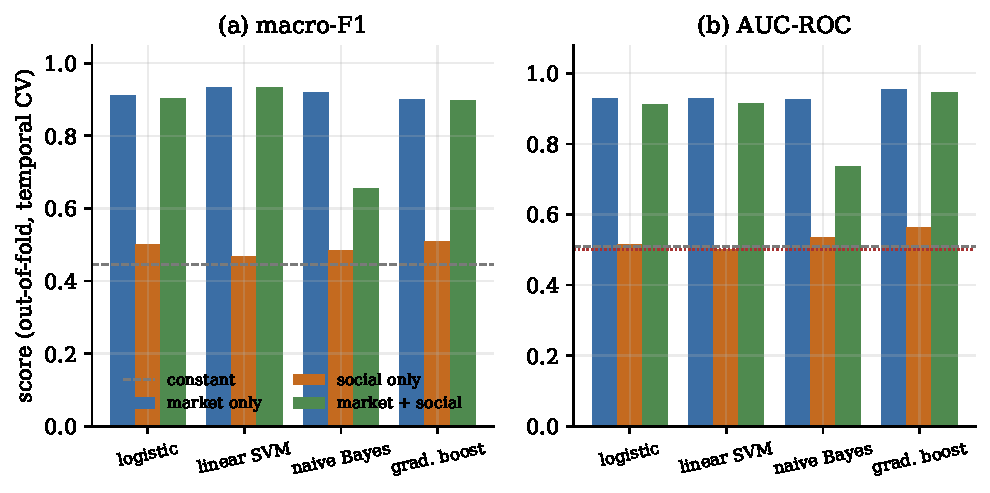
\includegraphics[width=\linewidth]{fig_task3_models.pdf}
\caption{Task-3 temporal-CV ablation. (a)~macro-F1 and (b)~AUC-ROC for each model family,
grouped by feature set (market only / social only / market\,+\,social). The market arm
(blue) dominates across every family; the social arm (orange) sits at the constant
baseline (grey dashed) and the chance line (red dotted); adding social to market (green)
yields no consistent gain.}
\label{fig:task3}
\end{figure}

\section{Complementary view: final pre-close backtest}
As a calibration-focused cross-check we also keep the Branch-09 single-cut backtest --- one
final pre-close prediction per contract, scored under 5-fold out-of-fold cross-validation
(\Cref{tab:results}, \Cref{fig:models}). It tells the same story from the probabilistic
angle: market-only attains Brier $0.031$ / AUC $0.989$, while market+social is slightly
\emph{worse} and social-only is below chance (AUC $0.404$).

\begin{table}[H]
\centering
\caption[Final pre-close backtest over 300 resolved contracts]{Final pre-close backtest
(5-fold out-of-fold; lower Brier/log loss, higher accuracy/AUC are better). The best
probabilistic score in each column is bold.}
\label{tab:results}
\small
\setlength{\tabcolsep}{5.5pt}
\begin{tabular}{@{}l r r r r r@{}}
\toprule
\textbf{Model} & \textbf{Brier}$\downarrow$ & \textbf{Log loss}$\downarrow$ &
\textbf{Accuracy}$\uparrow$ & \textbf{AUC}$\uparrow$ & \textbf{ECE}$\downarrow$\\
\midrule
base rate      & 0.154 & 0.486 & 0.810 & 0.487 & \textbf{0.003}\\
\rowcolor{pslight} market-only    & \textbf{0.031} & \textbf{0.110} & \textbf{0.963} & \textbf{0.989} & 0.020\\
social-only    & 0.160 & 0.504 & 0.810 & 0.404 & 0.060\\
market + social& 0.040 & 0.187 & 0.963 & 0.975 & 0.091\\
\midrule
\multicolumn{6}{@{}l}{\footnotesize\itshape Lift of market+social over market-only:\;
$\Delta\text{Brier}=-0.009$,\; $\Delta\text{LogLoss}=-0.077$ (both negative $=$ worse).}\\
\bottomrule
\end{tabular}
\end{table}

\begin{figure}[H]
\centering
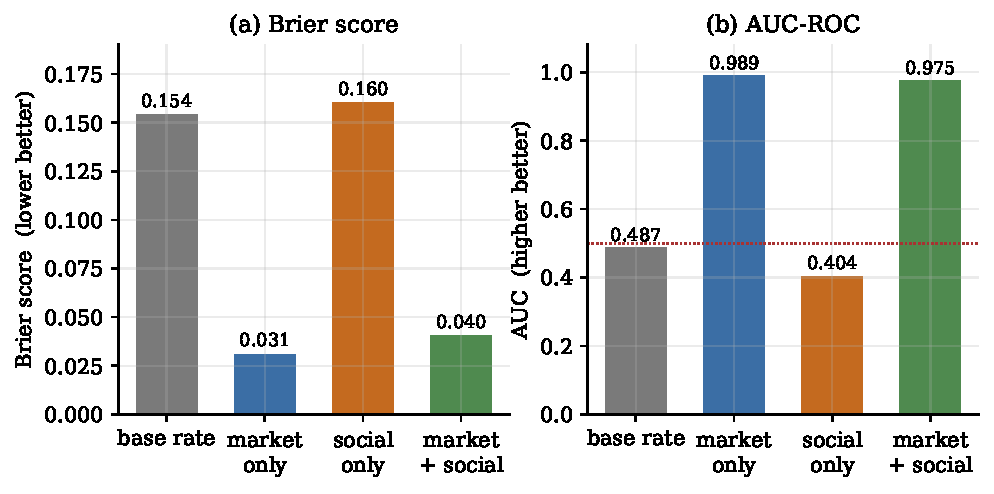
\includegraphics[width=\linewidth]{fig_model_comparison.pdf}
\caption{Final pre-close model comparison. (a)~Brier score and (b)~AUC. The market-only
baseline (blue) is the best model; adding social features (green) degrades it, and
social-only (orange) is no better than the chance line.}
\label{fig:models}
\end{figure}

\paragraph{Calibration.} \Cref{fig:calibration} shows the reliability of the two
price-based models. Market-only is well calibrated (ECE $0.020$): its predicted
probabilities match observed outcome frequencies closely, in the sense
of~\cite{niculescu2005predicting}. Market+social is visibly
\emph{less} calibrated (ECE $0.091$) --- the noisy social features push some
predictions away from the well-calibrated price.

\begin{figure}[H]
\centering
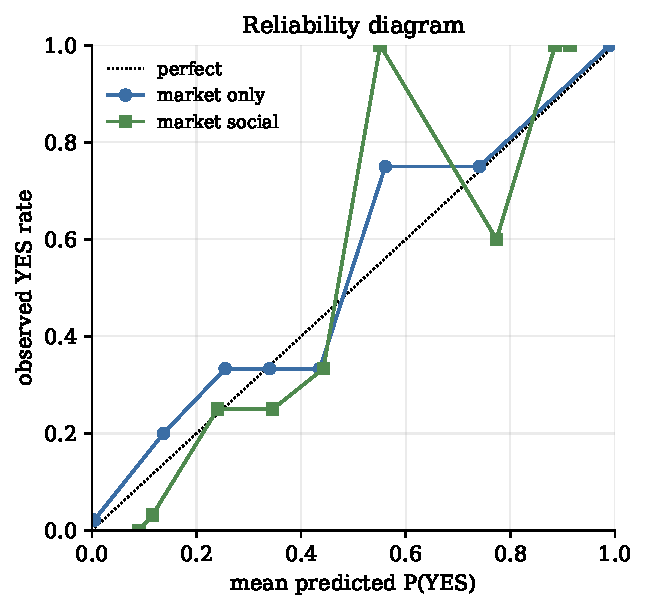
\includegraphics[width=0.5\linewidth]{fig_calibration.pdf}
\caption{Reliability diagram. The market-only model (blue) hugs the diagonal; adding
social features (green) worsens calibration.}
\label{fig:calibration}
\end{figure}

\paragraph{Why the combined model does not improve.} The fitted coefficients
(\Cref{fig:features}) tell the story compactly: the market-probability coefficient
($1.68$) dwarfs every social coefficient (all $|\beta|<0.10$). The model learns to trust
the price and to all but ignore the social features --- and the small weight it does put
on them adds variance, not signal.

\begin{figure}[H]
\centering
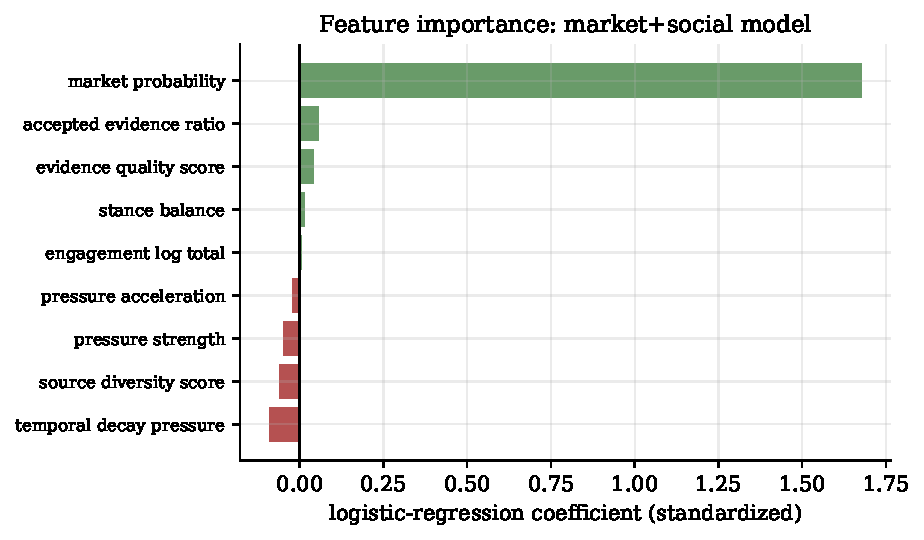
\includegraphics[width=0.72\linewidth]{fig_feature_importance.pdf}
\caption{Standardised logistic-regression coefficients of the market+social model. The
market probability dominates; the social features carry negligible, mixed-sign weight.}
\label{fig:features}
\end{figure}

\section{Does more evidence help? A coverage ablation}
A natural objection is that the social signal fails only because coverage is thin. We
test this by restricting the social-only model to the 73 contracts with
\emph{sufficient} accepted evidence. It does not rescue the signal: even there the model
predicts \textsc{No} for every contract, so its nominal AUC of $0.56$ reflects ranking
noise on an all-\textsc{No} classifier rather than usable signal; on the 227
insufficient-evidence contracts the AUC is $0.35$. The aggregate stance--outcome
correlation is $-0.015$ and the engagement-weighted net-pressure--outcome correlation is
$-0.013$ --- both indistinguishable from zero. \textbf{Within the range of coverage we have, more evidence
does not convert into predictive value}; the problem is the nature of the signal, not
merely its quantity (we revisit the quantity question, honestly, in
\Cref{ch:limitations}).

\begin{takeaway}
\textbf{Headline result.} Under expanding-window temporal cross-validation, all four
model families place the market arm at macro-F1 $0.90$--$0.93$ / AUC $0.93$--$0.95$,
while the social-only arm sits at near-chance macro-F1 $0.47$--$0.51$ (AUC $\approx0.5$)
and combining the two yields no consistent gain. The final pre-close backtest agrees:
market-only scores Brier $0.031$ / AUC $0.989$, adding social makes it \emph{worse}, and
social-only is below chance (AUC $0.404$). Social discourse adds \emph{no} incremental
predictive value over the Polymarket price in this dataset.
\end{takeaway}


%==============================================================================
\chapter{Discussion}
\label{ch:discussion}

The predictive result is negative and robust. This chapter explains \emph{why}, and
argues that the finding is informative rather than disappointing.

\section{Three structural causes}
\paragraph{1. The market is already efficient with respect to public information.}
By the efficiency argument of \Cref{ch:background}, any genuinely predictive public
signal tends to be arbitraged into the price. \Cref{sec:informative} quantified just how
strong that price already is --- AUC $0.90$ a full quarter before resolution. A public,
lagging social signal has essentially no room left to add value; the only edge would
come from \emph{private} or \emph{early} information, which broadcast Telegram channels
and public Reddit threads do not carry.

\paragraph{2. Social discourse is optimism-biased.}
Stance leans \textsc{Yes} $2.3{:}1$ while contracts resolve \textsc{No} $4.3{:}1$
(\Cref{fig:stance}), and on 58 of the 72 contracts where social pressure says
\textsc{Yes} the market resolves \textsc{No} (\Cref{fig:hype}). Discourse concentrates on
the exciting possibility that an event \emph{will} happen; markets, pricing base rates,
know that most such events do not. A signal that is systematically wrong in direction
cannot help a calibrated forecaster.

\paragraph{3. The discourse is reactive, not leading.}
The lead--lag analysis (\Cref{ch:correlation}) found no horizon at which social changes
precede price changes. Social media here narrates events the market has already priced; many candidate posts were
rejected by the temporal-admissibility filter for falling \emph{after} a contract had
already closed. A coincident-or-lagging signal cannot improve a forecast made before the
event.

\section{A note on coverage}
A fourth factor --- the channel/market mismatch (\Cref{ch:crossplatform}) --- limits how
much of the market the social layer even \emph{covers}: politics absorbs 81\% of
evidence, sports almost none. Crucially, though, the coverage ablation
(\Cref{sec:results}) shows that the failure is not merely one of quantity: even where
evidence is dense, its direction does not track outcomes. Broader coverage would let us
test more contracts, but on present evidence there is no reason to expect it to overturn
the direction of the result.

\section{Why a null result matters}
This is not a failed experiment; it is a clean, reproducible piece of evidence in a
literature crowded with fragile positive claims. It (i)~empirically corroborates the
informational efficiency of a major prediction market against a large, realistic social
corpus; (ii)~demonstrates a methodology --- leakage controls, ablation, calibration ---
that distinguishes genuine incremental value from spurious correlation; and (iii)~maps
precisely \emph{where} a social edge would have to come from (private/early signals,
information-asymmetric events) for future work to find it. ``PolySignal does not beat
Polymarket'' is, in this framing, exactly the finding.


%==============================================================================
\chapter{Limitations and Future Work}
\label{ch:limitations}

\section{Limitations}
We state the limitations plainly, since several of them bound the strength of the
conclusion.
\begin{description}[leftmargin=1.4em,style=nextline]
  \item[Platform coverage.] All three platforms are present in the analysed corpus, but
  it is \textbf{Telegram-dominated} (98.6\%), with a secondary Reddit contribution
  (1.2\%) and a small X/Twitter sample (0.2\%) whose scale is capped by X's
  anti-automation defences (\Cref{sec:scope}). The 68 Telegram channels are a purposive,
  not a random, sample, with a clear crypto/macro/geopolitics tilt. The predictive
  conclusions therefore hold for a Telegram-dominated corpus skewed towards
  crypto-adjacent discourse; whether a \emph{volume-balanced} three-platform corpus would
  change them is the central open question, and the architecture is built to answer it
  without code changes once such a corpus is available.
  \item[Domain coverage.] Sports contracts have almost no social evidence; the
  predictive conclusion is therefore strongest for politics and finance and weakest for
  sports.
  \item[Comments and authors.] Only a bounded \emph{sample} of per-comment text is
  collected, so comment-derived
  features are thin; broadcast Telegram channels expose neither follower counts nor
  author profile URLs, so those required fields are partially empty for that platform.
  \item[Deterministic baselines.] Linking and stance use deterministic heuristics; the
  optional cached LLM verifiers were not run at scale, which leaves $73\%$ of stance
  rows \code{neutral} and the heuristic NER noisy.
  \item[One prediction per contract.] Although we now score under expanding-window
  temporal cross-validation across contracts, each contract still contributes a single
  pre-close prediction; intra-contract time-sliced 7/3/1-day forecasts are deferred until
  the price/feature history is broad enough to support them cleanly.
  \item[Binary contracts only.] Multi-outcome markets are out of scope.
\end{description}

\section{Future work}
The limitations map directly to next steps, ordered by expected payoff:
\begin{enumerate}
  \item \textbf{Close the coverage gap.} Broaden the X/Twitter and Reddit passes (e.g.\
  via a paid research tier) and add sports-specific channels, so that all three platforms
  and all three domains carry \emph{comparable} evidence --- turning the cross-platform
  layer of \Cref{ch:crossplatform} into a volume-balanced three-platform complementarity
  test (Task~2.4).
  \item \textbf{Stronger stance and linking.} Run the cached LLM stance/relevance
  judges at scale and adopt the spaCy NER backend, reducing the neutral mass and the
  entity noise.
  \item \textbf{Time-sliced and early-signal evaluation.} Score 7/3/1-day pre-close
  windows and explicitly search for contracts where social \emph{leads} the price ---
  the only regime in which an edge is theoretically possible.
\end{enumerate}


%==============================================================================
\chapter{Conclusions}
\label{ch:conclusions}

We set out to determine whether social-media discourse adds predictive value over
Polymarket's own prices. To answer it we built an end-to-end Big Data pipeline that
collects 300 resolved binary contracts and their full-lifetime price series
($1{,}353{,}114$ points), collects a longitudinal multi-platform corpus
($1{,}368{,}041$ posts across Telegram, Reddit, and a small X/Twitter sample,
\Cref{sec:scope}), links posts to contracts with a deterministic semantic scorer,
enriches the text
with sentiment, entities, topics, and outcome-aware stance, projects everything into a
Neo4j knowledge graph, and condenses the evidence into a per-market Social Pressure
Index that feeds a leakage-controlled backtest --- all exposed through an interactive
dashboard. The system satisfies each requirement of Tasks~1, 2, and the optional
Task~3.

The descriptive study confirmed that Polymarket prices are already highly informative of
outcomes and become more so as resolution nears (AUC $0.90\!\to\!0.99$). The predictive
study returned a clear, well-controlled \textbf{null result} that is robust across four
model families under expanding-window temporal cross-validation: the market arm reaches
macro-F1 $0.90$--$0.93$ and AUC up to $0.95$, the social-only arm never escapes
near-chance (macro-F1 $\approx0.5$), and combining the two adds no consistent lift; the
final pre-close backtest concurs (market-only Brier $0.031$ / AUC $0.989$, market+social
\emph{worse}, social-only below chance). We traced this to the market's informational
efficiency, a systematic optimism bias in
social stance, the reactive (non-leading) nature of the discourse, and a structural
mismatch between the available channels and the contract sample.

The contribution of this work is therefore twofold: a reproducible, leakage-aware
methodology for studying social signals against prediction markets at scale, and the
honest empirical finding that public social discourse does not, in this setting, beat
the market price. In a field prone to over-claiming, demonstrating \emph{where} and
\emph{why} a signal fails --- and doing so reproducibly --- is a result worth reporting.


%------------------------------------------------ APPENDIX
%==============================================================================
%  APPENDICES
%  A: Reproducibility and how to run   |   B: AI-assisted development
%==============================================================================
\appendix

\chapter{Reproducibility and How to Run}
\label{ch:reproduce}
The project is self-contained and portable: it targets \textbf{Python~3.11+}, declares
every dependency in \code{pyproject.toml}, and the dashboard runs fully offline from the
persisted pipeline artifacts --- \emph{no API keys and no internet access are required}
to reproduce the figures, tables, and the interactive app in this report. Secrets live
only in an untracked local \code{.env}; the shared \code{.env.example} is a blank
template. The steps below reproduce the deliverable on a clean machine.

\paragraph{1. Create an isolated environment and install.}
The core install is enough to launch the dashboard and run the figure/test suite; the
bracketed extras add the optional collectors and developer tooling.
{\small\begin{verbatim}
python -m venv .venv
# Windows:        .venv\Scripts\activate
# macOS / Linux:  source .venv/bin/activate
pip install -e .                          # core: dashboard + analysis
pip install -e ".[dev,nlp,telegram,scraping]"   # everything (optional)
\end{verbatim}}

\paragraph{2. Launch the interactive dashboard.}
A single command builds the served payload from the artifacts in \code{data/} and opens
the browser on a local, zero-dependency origin (CORS-free, no external calls).
{\small\begin{verbatim}
python scripts/serve_app.py        # cross-platform
run_app.cmd                        # Windows one-click equivalent
# -> http://127.0.0.1:8000/
\end{verbatim}}

\paragraph{3. Regenerate every figure and table.}
All quantitative results are derived from the persisted artifacts by a single released
step, so nothing in this report is hand-transcribed.
{\small\begin{verbatim}
python scripts/_paper_stats.py     # refresh the stats JSONs from data/
python scripts/_paper_figs.py      # writes pdf_latex/figures/*.pdf
pytest                             # run the test suite (757 passing)
polysignal --help                  # explore the pipeline CLI
\end{verbatim}}

\paragraph{4. (Optional) rebuild the report PDF.}
The \code{pdf\_latex/} folder compiles with any standard TeX toolchain --- \code{pdflatex
+ bibtex}, \code{latexmk}, \code{tectonic}, or Overleaf --- using only standard packages.
{\small\begin{verbatim}
cd pdf_latex && latexmk -pdf main.tex     # or: tectonic main.tex
\end{verbatim}}

\noindent\textbf{What the release bundle contains.} The publishable archive ships the
source (\code{src/}, \code{scripts/}, \code{webapp/}, \code{tests/}), the report
(\code{pdf\_latex/} with \code{main.pdf}), the documentation (\code{docs/}), and the
\emph{minimal} set of \code{data/} artifacts the dashboard reads (timelines, social
pressure, stance labels, accepted evidence, market metadata, post enrichment, and the
analytics/backtest summaries --- about 60\,MB). The multi-gigabyte raw corpus, caches,
virtual environment, and portable tool downloads are deliberately excluded; they are
regenerable and carry no analytical value beyond what the shipped artifacts already
summarise.


\chapter{AI-Assisted Development: Tools and Repositories}
\label{ch:aitools}
In the interest of transparency, this appendix documents the AI-assisted development
workflow behind PolySignal. The \emph{scientific} results are independent of it --- every
number in this report is regenerated deterministically from the persisted artifacts
(\Cref{ch:reproduce}), and no AI agent ever produced a result: the agents wrote
\emph{code}, the code produced the artifacts, and the artifacts produced every figure and
table. What the AI workflow bought was engineering throughput \emph{with} discipline.

\section{AI coding assistants}
Three command-line coding agents were used in deliberately complementary roles, so that
no single model's blind spots went unchecked:
\begin{description}[leftmargin=1.4em,style=nextline]
  \item[Claude Code (Anthropic).] The primary agent for implementation, refactoring, and
  this report. It carried the bulk of the pipeline --- ingestion, contract--post linking,
  outcome-aware stance, the Social Pressure Index, and the leakage-controlled backtest ---
  drove the test-first workflow, and authored and revised the \LaTeX{} of this document.
  \item[Codex (OpenAI).] A second pair of eyes for focused code generation and
  cross-checking: alternative implementations of tricky functions, and independent review
  of edge cases and failure modes.
  \item[Gemini CLI (Google).] Used for large-context sweeps across the codebase and for
  corroborating design decisions, providing a third independent perspective on
  architecture and data-handling choices.
\end{description}
Running three independent agents --- rather than trusting one --- turned model
disagreement into a useful signal: where they agreed we proceeded with confidence; where
they diverged, the divergence flagged exactly the spots that warranted a human decision.

\section{Supporting repositories and tooling}
\begin{description}[leftmargin=1.4em,style=nextline]
  \item[ECC --- a comprehensive ``everything Claude Code'' framework.] ECC is an open
  repository --- the winning entry of a 2026 hackathon --- that packages a complete Claude
  Code setup: agent definitions, multi-agent orchestration rules, reusable skills and
  commands, and a full set of engineering conventions (coding style and immutability, a
  mandatory test-coverage bar, security checks against hard-coded secrets and unvalidated
  input, and a code-review gate before any change is accepted). We adopted ECC to drive
  and standardise the agentic workflow; it is what kept three different agents producing
  consistent, reviewable code rather than three divergent styles, and why the repository
  ships with \textbf{757 passing tests} and a uniform module layout.
  \item[Graphify.] A repository-graph tool (configured through \code{.graphifyignore},
  output under \code{graphify-out/}) that builds a navigable map of the codebase --- its
  modules, symbols, and their relationships. It gave the agents structural context for
  navigating a large repository, so edits respected the existing architecture
  (\Cref{ch:architecture}) instead of reinventing it.
\end{description}

\section{How the tools were leveraged}
The workflow composed these pieces into a single loop: plan a change with one agent,
implement it test-first, cross-review it with a second agent, and keep every change behind
the ECC review-and-coverage gate, using the Graphify map to land edits in the right place.
The result is a large, well-tested, well-documented codebase and a fully reproducible
report, produced quickly but without surrendering the scientific honesty that is the whole
point of a null-result study. The AI tooling accelerated the \emph{engineering}; the
\emph{evidence} remains entirely the data's.


%------------------------------------------------ BIBLIOGRAPHY
\cleardoublepage
\addcontentsline{toc}{chapter}{Bibliography}
\bibliography{references}

\end{document}
